%!TEX encoding = UTF-8 Unicode

\documentclass[12pt,a4paper]{report}

\usepackage{dolgozat}

\usepackage{hyperref}

\usepackage{listings}
\usepackage{python}
\usepackage{cpp}

\usepackage{verbatim}
%\usepackage{relsize}

% \usepackage{tikz}

\usepackage{pgf-pie}

\usepackage{pgfplots}
\pgfplotsset{width=7cm,compat=1.8}
\pgfmathdeclarefunction{gauss}{2}{
  \pgfmathparse{1/(#2*sqrt(2*pi))*exp(-((x-#1)^2)/(2*#2^2))}%
}

%\linespread{1.2}

\begin{document}

%% !TEX encoding = UTF-8 Unicode


\pagestyle{empty} %a címlapon ne legyen semmi=empty, azaz nincs fejléc és lábléc

\begin{flushleft}
\textsc{\bfseries Miskolci Egyetem}\\
Gépészmérnöki és Informatikai Kar\\
Analízis Intézeti Tanszék
\end{flushleft}

%A fõiskola logoja
{\large
\begin{center}
\vglue 1truecm
\textbf{\huge\textsc{Szakdolgozat}}\\
\vglue 1truecm

\epsfig{file=cimlap/ME_logo.eps, width=4.8truecm, height=4truecm}\\
\textbf{\textsc{Miskolci Egyetem}}
\end{center}}

\vglue 1.5truecm %függõleges helykihagyás

%A szakdolgozat címe, akár több sorban is
{\LARGE
\begin{center}
\textbf{Félkész- és késztermék nyilvántartó rendszer fejlesztése}
\end{center}}

\vspace*{2.5truecm}
%A hallgató neve, évfolyam, szak(ok), a konzulens(ek) neve
{\large
\begin{center}
\begin{tabular}{c}
\textbf{Készítette:}\\
Bányi Attila\\
Gazdaságinformatikus BSc
\end{tabular}
\end{center}
\begin{center}
\begin{tabular}{c}
\textbf{Témavezető:}\\
Dr. Hriczó Krisztián\\
egyetemi adjunktus, PhD
\end{tabular}
\end{center}}
\vfill
%Keltezés: Hely és év
{\large
\begin{center}
\textbf{\textsc{Miskolc, 2018}}
\end{center}}

\newpage

\pagestyle{empty}
%% !TEX encoding = UTF-8 Unicode

%Feladatkiiras
\begin{flushleft}
\textsc{\bfseries Miskolci Egyetem}\\
Gépészmérnöki és Informatikai Kar\\
Alkalmazott Matematikai Intézeti Tanszék\hspace*{4cm}\hfil \textbf{Szám:}
\end{flushleft}
\vskip 0.5cm
\begin{center}
\large\textsc{\bfseries Szakdolgozat Feladat}
\end{center}
\vskip 0.5cm
Bányi Attila (DURITT) gazdaságinformatikus.\newline

\noindent\textbf{A szakdolgozat tárgyköre:} Adatbáziskezelés, Objektum-orientált programozás\newline

\noindent\textbf{A szakdolgozat címe:} Félkész- és késztermék nyilvántartó rendszer fejlesztése\newline

\noindent\textbf{A feladat részletezése:}

\bigskip

Adatbázisfejlesztés félkész- és késztermékek nyilvántartására. Az adatbázisból lekérdezhető a termék bekerülési ideje, gyártója, értéke, stb. Az adatbázis specifikálható legyen termelő/kereskedő vállalat számára. Grafikus felhasználói felület létrehozása az adatbázis kezeléséhez.

\vfill

\noindent\textbf{Témavezetõ:} Dr. Hriczó Krisztián (egyetemi adjunktus, PhD) \newline

\noindent\textbf{A feladat kiadásának ideje:}
2018. február 27.
\newline

%\noindent\textbf{A feladat beadásának határideje:}

\vskip 2cm

\hbox to \hsize{\hfil{\hbox to 6cm {\dotfill}\hbox to 1cm{}}}

\hbox to \hsize{\hfil\hbox to 3cm {szakfelelõs}\hbox to 2cm{}}

\newpage

\vspace*{1cm}  
\begin{center}
\large\textsc{\bfseries Eredetiségi Nyilatkozat}
\end{center}
\vspace*{2cm}  

Alulírott \textbf{Bányi Attila}; Neptun-kód: \texttt{DURITT} a Miskolci Egyetem Gépészmérnöki és Informatikai Karának végzõs gazdasági informatikus szakos hallgatója ezennel büntetõjogi és fegyelmi felelõsségem tudatában nyilatkozom és aláírásommal igazolom, hogy
\textit{Félkész- és késztermék nyilvántartó rendszer fejlesztése}
címû szakdolgozatom/diplomatervem saját, önálló munkám; az abban hivatkozott szakirodalom
felhasználása a forráskezelés szabályai szerint történt.\\

Tudomásul veszem, hogy szakdolgozat esetén plágiumnak számít:
\begin{itemize}
\item szószerinti idézet közlése idézõjel és hivatkozás megjelölése nélkül;
\item tartalmi idézet hivatkozás megjelölése nélkül;
\item más publikált gondolatainak saját gondolatként való feltüntetése.
\end{itemize}

Alulírott kijelentem, hogy a plágium fogalmát megismertem, és tudomásul veszem, hogy
plágium esetén szakdolgozatom visszautasításra kerül.

\vspace*{3cm}

\noindent Miskolc, \hbox to 2cm{\dotfill} év \hbox to 2cm{\dotfill} hó \hbox to 2cm{\dotfill} nap

\vspace*{3cm}

\hspace*{8cm}\begin{tabular}{c}
\hbox to 6cm{\dotfill}\\
Hallgató
\end{tabular}

\newpage

\linespread{0.8}

\noindent 1.

\begin{tabular}{cl}
&szükséges (módosítás külön lapon) \\
A szakdolgozat feladat módosítása& \\
& nem szükséges\\
&\\
\hbox to 4cm{\dotfill}&\multicolumn{1}{c}{\hbox to 5cm{\dotfill}}\\
dátum& \multicolumn{1}{c}{témavezetõ(k)}
\end{tabular}
\vskip1.5mm

\noindent 2. A feladat kidolgozását ellenõriztem:

\vskip1.5mm

\begin{tabular}{l@{\hspace*{4cm}}l}
témavezetõ (dátum, aláírás):& konzulens (dátum, aláírás):\\
\dotfill&\dotfill\\
\dotfill&\dotfill\\
\dotfill&\dotfill
\end{tabular}

\vskip1.5mm

\noindent 3. A szakdolgozat beadható:

\vskip1.5mm

\begin{tabular}{@{\hspace*{1.3cm}}c@{\hspace*{2.1cm}}c}
\hbox to 4cm{\dotfill}&\multicolumn{1}{c}{\hbox to 5cm{\dotfill}}\\
dátum& \multicolumn{1}{c}{témavezetõ(k)}
\end{tabular}

\vskip1.5mm

\noindent 4.
\begin{tabular}[t]{@{}l@{\hspace*{1mm}}l@{\hspace*{1mm}}l@{}}
A szakdolgozat& \hbox to 3.5cm{\dotfill} &szövegoldalt\\
              & \hbox to 3.5cm{\dotfill} &program protokollt (listát, felhasználói leírást)\\
              &\hbox to 3.5cm{\dotfill}   &elektronikus adathordozót (részletezve)\\
              &\hbox to 3.5cm{\dotfill} & \\
              &\hbox to 3.5cm{\dotfill} &egyéb mellékletet (részletezve)\\
              &\hbox to 3.5cm{\dotfill} &\\
\end{tabular}
\newline tartalmaz.

\vskip1.5mm

\begin{tabular}{@{\hspace*{1.3cm}}c@{\hspace*{2.1cm}}c}
\hbox to 4cm{\dotfill}&\multicolumn{1}{c}{\hbox to 5cm{\dotfill}}\\
dátum& \multicolumn{1}{c}{témavezetõ(k)}
\end{tabular}

\noindent 5.

\begin{tabular}{ll}
&bocsátható\\
A szakdolgozat bírálatra& \\
& nem bocsátható\\
\end{tabular}

\vskip1.5mm

\noindent A bíráló neve: \hbox to 8cm{\dotfill}

\vskip4mm

\begin{tabular}{@{\hspace*{1.3cm}}c@{\hspace*{2.1cm}}c}
\hbox to 4cm{\dotfill}&\multicolumn{1}{c}{\hbox to 5cm{\dotfill}}\\
dátum& \multicolumn{1}{c}{szakfelelõs}
\end{tabular}

\noindent 6.
\begin{tabular}[t]{@{}l@{\hspace*{1mm}}l@{\hspace*{1mm}}l@{}}
A szakdolgozat osztályzata& &\\
&a témavezetõ javaslata:& \hbox to 3cm{\dotfill}\\
&a bíráló javaslata:& \hbox to 3cm{\dotfill}\\
&a szakdolgozat végleges eredménye:& \hbox to 3cm{\dotfill}
\end{tabular}

\vspace*{4mm}

\noindent Miskolc, \hbox to 4.5cm{\dotfill} \hspace*{2.5cm}
\begin{tabular}[t]{cc}
\hbox to 6cm{\dotfill}\\
a Záróvizsga Bizottság Elnöke
\end{tabular}

\linespread{1.2}


\cleardoublepage
\pagenumbering{gobble}
\tableofcontents
\cleardoublepage
\pagenumbering{arabic}

\newpage

\linespread{1.2}
\pagestyle{fancy}

% !TEX encoding = UTF-8 Unicode

\Chapter{Bevezetés}

\hspace{12.5mm}Szakdolgozatom célja egy termelő- és kereskedő vállalatok számára specializálható, grafikus felhasználói felülettel rendelkező adatbáziskezelő szoftver létrehozása volt, amellyel az említett vállalkozások raktározási és logisztikai ügyeit egyszerűen, átláthatóan, megelőző informatikai ismeretek nélkül is lehessen kezelni, azon a logikán alapulva, amit korábban papíron alkalmaztak.

% elméleti jelentőség

\setlength{\parindent}{12.5mm}Az alkalmazás elméleti jelentősége az iránymutatás a vállalatok részére, hogy a jelenleg is zajló, negyedik ipari forradalom jegyében lépjenek előre, és zárkózzanak fel a digitális technológia vívmányaival karöltve a hatékonyabb és kevesebb emberi munkavégzés érdekében, a logisztika, raktározás és a valós időben történő nyomkövetés használatával, akár személyi számítógépeken, akár mobil eszközökön. Megelőző kutatásaim és személyes tapasztalataim alapján tisztában vagyok vele, hogy digitális bevándorlóként sokkal nehezebb átlátni és megérteni egy számítógépes program működését, de éppen ezért támasztottuk a programmal szemben azt az alapvető követelményt, hogy könnyen értelmezhető, felhasználóbarát kezelőfelülettel rendelkezzen, úgy, hogy egy informatikában kevésbé jártas személy is megfelelően tudja használni.

% gyakorlati jelentőség

\setlength{\parindent}{12.5mm}A szoftver gyakorlati jelentősége az előző pontban említett elméleti előrelépés alkalmazása esetén valósul meg. A digitális átállás jelentősen leegyszerűsíti és felgyorsítja a munkát, valamint a digitális munkavégzés által csökkentett papírhasználat környezetbarát is.

% jelentőség rám nézve

\setlength{\parindent}{12.5mm}Szakdolgozatom elméleti és gyakorlati jelentősége rám tekintve, hogy az eddig tanult, jellemzően fiktív adatokra épülő szoftveres megoldásokat már létező, valós problémakörre tudtam kiterjeszteni. Ehhez nagyban hozzájárult az, hogy az egyetemi alapképzés kereteiben megfelelő szintű tudást sajátítottam el ahhoz, hogy valós adatokkal dolgozó szoftvereket készítsek, amik gyakran nagy felelősséggel járnak.
% !TEX encoding = UTF-8 Unicode

\Chapter{Követelmények és környezet}


\hspace{12.5mm}A Földön élő emberek túlnyomó része rendelkezik valamilyen infokommunikációs eszközzel és a teljes lakosság 53,6\%-a kapcsolódik az internethez. Ez az arány a Földet tekintve csekélynek mondható, különösképp azért, mert jelenleg már a negyedik ipari forradalom zajlik, de az érték azért ilyen alacsony, mert az ún. fejletlen-, fejlődő- és fejlett országok között óriási technológiai és fejlettségi szakadékok vannak. Afrikában ez az arány 18\%, itt az emberek általában iskolákban, egyetemeken, nyilvános helyeken vagy közösségi házakban férnek hozzá az internethez, míg Európában ez az érték 84,2\%, tehát már a ,,veteránok'' és a ,,baby-boomerek'' között is jócskán akadnak, akik alkalmazzák a technológiát, még akkor is, ha ők a legmesszebbről érkezett digitális bevándorlók \cite{itu_ict_fac_fig_2017}.\par

\setlength{\parindent}{12.5mm}Az Európai Unió több tagállamában, többek közt Magyarországon is kötelezővé vált az elektronikus számlázás, így a vállalkozásnak rendelkeznie kell egy  elektronikus számlát kezelő és kibocsátó szoftverrel \cite{nav_online_szla}, ám ez még nem jelenti azt, hogy minden vállalkozás tulajdonában van olyan alkalmazás is, amellyel a nyilvántartást, logisztikát hatékonyan tudják kezelni. Mivel a világ elindult az egységes digitalizáció útján - nem csak a szórakozás, hanem a munkavégzés terén is -, és a tendencia is jó irányba halad, ezért egy átlátható és hatékony megoldást hoztam létre a fejlődés útjára lépő vállalkozások számára.\par

\setlength{\parindent}{12.5mm}Az adatmodellek, sémák és az üzleti logika kalakításakor több meglévő, nem digitális alapon működő nyilvántartást vettem alapul, így az átállás nem jár a meglévő készletek jelentős átcsoportosításával, esetleg néhány kisebb, logikai változás történik. A kezdeti adatfeltöltés időigényes művelet, de használat közben rövid időn belül belátják majd, hogy a jól strukturált adatkezelés, a gyors válaszidők, a hatékony keresési és szűrési funkciók jelentősen felgyorsítják és hatkonyabbá teszik a munkavégzést, hamar megtérül az adatbevitelbe fektetett idő és energia.\par

\setlength{\parindent}{12.5mm}Az adatbáziskezelő szoftver jelenleg a termelő- és kereskedő vállalatok részére specializált, de az alapvető üzleti logika és szoftveres megoldás nem csak ezen területnek felel meg, így igény szerint más területen is alkalmazható, többek közt szolgáltató, pénzügyi, fuvarozó, vendéglátó és logisztikai vállalatoknál is. A szoftverbe és az adatbázisba implementált eljárások a megrendelő igénye szerint paraméterezhetőek, maximálisan a vállalat működésére szabható megoldások létrehozásával.\par


\Section{Követelmények}

A szoftverrel szemben támasztott alapvető követelmények:
\begin{itemize}
\item grafikus megjelenési felület,
\item könnyen értelmezhető, felhasználóbarát megjelenés,
\item gombok és menük alkalmazása, parancssor mellőzése
\item egy adatbázissal történő valós idejű, oda-vissza irányú kommunikáció,
\item az adatbázishoz kapcsolódás felhasználónévvel és jelszóval történő védelme (beléptetőrendszer),
\item felkész- és késztermékek közös táblában történő tárolása, megkülönböztetésük egy mező értékével,
\item bekerülési (bruttó) árból számított nettó, eladási és akciós ár számítása előre meghatározott matematikai képletekkel,
\item a számított értékek védettsége,
\item tetszés szerint választható „akciós” termékek nyilvántartása és lehetőség csak ezen termékek megjelenítésére,
\item események részletes naplózása,
\item napló védelme (utólag nem módosítható, nem törölhető),
\item a megjelenített adatok közötti, egyszerre több érték szerinti szűrésének lehetősége,
\item keresés az adatbázis elemei közt, egyszerre több mező értékének figyelembevételével,
\item a megjelenített adatok tetszés szerinti rendezésének lehetősége,
\item a megjelenített táblázatok futási időben történő, tetszés szerinti átrendezése,
\item a felhasználó által bevitt adatok ellenőrzése mind adatbázis, mind szoftver oldalról,
\item esetleges helytelen/hibás beviteli adatok esetén a hibás mező(k) jelölése, segítség a helyes szintaktikához,
\item a program, az adatbázis és az adatkapcsolat által létrejött hibák kezelése.
\end{itemize}
\newpage

\Section{Környezet}
A fejlesztés kezdetén logikailag kellett megterveznem a szoftver működését, és ennek megfelelően kellett megválasztanom a hozzá szükséges környezetet. Ez magában foglalja a futtató operációs rendszert, a fejlesztés során használt programozási nyelvet, a futtatáshoz szükséges keretrendszert, a fejlesztői környezetet, valamint az adatbáziskezelő rendszert. Mivel Magyarországon az elmúlt egy évben és azt megelőzően is magabiztosan uralja a piacot a Microsoft Windows operációs rendszere \cite{statcounter_os_market_share}, valamint saját munkáimra és tanulmányaim alatt is jellemzően ezt az operációsrendszert használtam, így a választásom egyértelmű volt.

\SubSection{C\#}
A program készítésekor C\# nyelvet használtam, választásom azért esett erre, mert már egyetemi tanulmányaim előtt is használtam ezt a nyelvet, és a BSc alatt is ez volt a választott objektum-orientált programozási nyelvem, valamint a témavezetőm és általam kijelölt célok megvalósítására is alkalmas.\par
A C\# egy erősen típusos, normatív, objektum-orientált programozási nyelv, amelynek alapjául a C++ és a Java szolgált. A fejlesztéskor a Microsoft a C++ hatékonyságát, a Visual Basic kezelhetőségét és a Java platform-függetlenségét próbálta ötvözni, amely sikerült is, 2000-ben, a Professional Development Conference-en mutatták be először a nyilvánosság előtt, és megjelenése óta már a hetedik verziónál jár. Minden verzió számos újítással érkezett, többek között a párhuzamos programozás támogatásával. Megjegyzendő, hogy a C\# fejlesztésének vezetője a kezdetektől az az Anders Hejlsberg, aki a Turbo és Borland Pascal, valamint a Delphi létrehozásakor főmérnökként dolgozott a Borlandnál. A nyelv olyan széles körben alkalmazott, hogy néhány hónappal megjelenése után, 2001 decemberében már szabványosították, erről az Európai informatikai és kommunikációs rendszerek szabványosítási szövetsége ECMA-334 \cite{ecma_334_c_sharp} kódnévvel ellátott publikációjában olvashatunk, valamint 2003 óta ISO szabvány is lett, erről jelenleg a Nemzetközi Szabványügyi Szervezet ISO/IEC 23270:2006 \cite{iso_iec_c_sharp_2006} szabványának hivatalos kiadványában találunk bővebb információt, de a köeljövőben felváltja majd egy új változat, ami a kurrens újításokat is tartalmazza, ez a későbbiekben ISO/IEC DIS 23270 \cite{iso_iec_dis_c_sharp_future} néven lesz megtalálható .\par

\SubSection{.NET Core Command-Line Interface (CLI)}
A már említett, 2000-es Professional Development Conference-en a C\#-pal együtt a .NET Core Command-Line Interface (a továbbiakban .NET) keretrendszer is megjelent, ami alapfeltétel a C\#-ban írt programok futtatásához. A Visual Studio 6.0 megjelenése óta a Microsoft nem a Win32 környezetben, hanem a .NET környezetben futtatja programjait, utalva ezzel a hálózati munka integrálására, amit az általam készített program is használ. A keretrendszer a használt fejlesztőkörnyezetnek fordítási idejű szolgáltatásokat végez, és az így lefordított alkalmazásoknak futási idejű környezetet biztosít, valamint az alkalmazások számára a már nem használt objektumok memóriabeli felszabadítását automatikusan elvégzi a Garbage Collector (szemétgyűjtő) használatával. A fordító a forráskódot nem natív, hanem egy köztes kódra fordítja le. Ez a köztes kód az MSIL (Microsoft Intermediate Language), ezt továbbfejlesztve, a Visual Studio 2015-ben hivatalosan is megjelent a .NET Compiler Platform (Roslyn), ami a Visual Basic-hez és C\#-hoz készült új, fordítói platform, ami közvetlenül a kódanalízist szolgálja, valamint készíthető vele különálló Form alkalmazás, amely a forráskódkezelő eszközökhöz kapcsolódva forráskódok megfigyelésére, statisztikáinak létrehozására használható.\par

A keretrendszer az alkalmazások típusai szerint több csoportba sorolja az osztálykönyvtárakat, most csak azokat említem, amelyeket érint az alkalmazásom:
\begin{itemize}
\item ADO.NET: Adatbázisrendszerek, és a hozzájuk tartozó driverek menedzselése és használata, valamint az adatkapcsolat kiépítése és működtetése
\item Windows Form: Windows alapú felhasználói könyvtár, grafikus felhasználói felülettel rendelkező ablakok létrehozásához
\end{itemize}
A .NET keretrendszert is szabványosították Common Language Infrastructure (CLI) néven, ez az Európai informatikai és kommunikációs rendszerek szabványosítási szövetségénél az ECMA-335 kódnevet kapta \cite{ecma_335_cli_dotnet} és a Nemzetközi Szabványügyi Szervezet az ISO/IEC 23271:2012 \cite{iso_iec_cli_dotnet_2012} kódszámmal jelölte, amikből egyértelműen látszik, hogy a C\# és .NET szoros kapcsolatban állnak, kódszámaik közvetlenül egymást követik.

A szoftver futtatásához szükséges, feljebb említett keretrendszer a Windows Update-ből, és a MSDN-ről is elérhető, valamint a mellékelt lemezen is megtalálható a jelenleg legújabb, 4.7.2 verzió offline telepítője az \texttt{InstallMeFirst\textbackslash NET472} könyvtárban, \texttt{NDP472-KB4054530-x86-x64-AllOS-ENU.exe} néven.\par

\SubSection{Microsoft Visual Studio 2015 Update 3}
Elsősorban az objektum-orientált szemléletmód és az Oracle adatbázissal történő megfelelő, robosztus működés volt a szempont a fejlesztői környezet kiválasztásakor. A környezet és a driverek megfelelő beállításainak elvégzése után a kapcsolat szilárd és a Visual Studio is megfelelően kezel minden, Oracle-lel kapcsolatos metódust.\par
A Visual Studio 2015 már több, mint 15 nyelvet támogat, és már nem csak Windows platformra lehet fejleszteni, hanem többek közt Azure, Android, iOS rendszerekre is, amellyel a alkalmazásom továbbgondolása esetén, és a jelenleg zajló negyedik ipari forradalom jegyében az adatbázis (legyen szó konkrétan készletezésről, leltárról, vagy bármilyen logisztikai műveletről) egy mobil eszközről elérhető úgy, hogy közben a felhasználó fizikailag ott van a raktárban, és az eszköz segítségével, egyedi azonosítókat használva valós időben, valós adatokkal dolgozhat, ide értve a készletfeltöltést – akár vonalkód szkenneléssel –, ellenőrzést, keresést, kivételezést.\par

\SubSection{SQL}
Az SQL (Structured (English) Query Language) egy struktúrált, kötött szintaxisú, angol kulcsszavakon alapuló (nem csak) lekérdező programnyelv, amelyet minden jelentősebb relációs adatbáziskezelő rendszer használ (Microsoft SQL, Oracle Database, MySQL, PostgreSQL) \cite{kovacs_laszlo_adatbazisok}. A nyelvet a webes alkalmazások mellett számos PC-n futó adatbáziskezelő is alkalmazza, a nyelv olyan gyorsan bővül és fejlődik, hogy a jelenleg legújabb, ISO/IEC 9075:2016 \cite{iso_iec_sql} szabvány az azt megelőzőhöz képest öt év alatt 44 új funkcióval bővült \cite{whats_new_in_sql}.


\SubSection{Oracle Database Express Edition 11g Release 2}
Az Oracle Database Express Edition az Oracle egyik ingyenes relációs adatbáziskezelője, amely nem csak konzolos, hanem webes interfésszel is rendelkezik, így a fejlesztés is könnyebb, és a felhasználók is relatíve könnyen, egyszerűen kezelhetik az adatbázist. Néhány adminisztrációval kapcsolatos feladathoz szükséges némi parancssori ismeret, de mivel a szoftver kiváló dokumentációkkal rendelkezik, az esetleges nehézségek is megoldhatóak. Mivel az Oracle rendelkezik olyan illesztőprogramokkal, amelyek a fejlesztőkörnyezettel kommunikálnak, így a webes felület elhagyható, elegendő egy ablakban történő kliens-szerver kapcsolat is, amely mellett - többek közt – a jóval kisebb memóriahasználat és az alacsonyabb erőforrásigény szól.\par
A tanulmányaim alatt az Adatbáziskezelés I-II. tantárgyakból az Oracle Database Express Edition adatbáziskezelő rendszert használtam, így számos funkcióját megismerhettem, megtanultam a kliens oldal használatát, különböző eljárásokat. A szakdolgozatomhoz szükséges szerver oldal konfigurációját pedig magam kellett elsajátítanom, a rendelkezésre álló dokumentációból (megjegyzendő, hogy az Oracle dokumentációi kiemelkedően jók és részletesek), így végül egy jól működő rendszert tudtam használni úgy, hogy mind a szerver, mind a kliens oldal működését a megfelelő szinten elsajátítottam.\par



% !TEX encoding = UTF-8 Unicode

\Chapter{Grafikus megjelenés}

\hspace{12.5mm}A program működése során két fő ablakkal találkozhatunk, az egyik - és megjelenési sorrendben az első - egy bejelentkező ablak (LoginForm), a másik pedig maga a grafikus felületű adatbáziskezelő (MainForm).  Ezen kívül találkozhatunk még felugró ablakokkal, ezek jellemzően valamilyen információ megjelenítése esetén vagy hibák kezelésekor jelennek meg, de ezek programozástechnikailag ún. üzenetdobozok (MessageBox), nem a klasszikus ablakok (Form), mivel ezek tájékoztatást adnak egy adott eseményről.

\Section{Belejentkező ablak}
\label{loginform}

A program indulásakor egy $350 \times $250 pixel méretű, átméretezést, teljes- és kis méretbe helyezést nem engedélyező bejelentkező ablak jelenik meg, ahol az inicializálás során két mező, egy legördülő menü, valamint egy gomb jön létre. Az első két mező a felhasználónév és a hozzá tartozó jelszó beírására szolgál, a legördülő menüből pedig kiválaszthatjuk a kiszolgálót, ez látható a \ref{fig:loginForm_connChoices} ábrán.


\begin{figure}[ht]
\centering
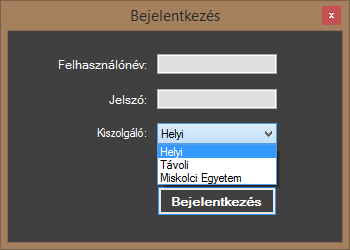
\epsfig{file=kepek/loginForm_connChoices.png, scale=0.8}
\caption{A bejelentkező ablak (LoginForm)} 
\label{fig:loginForm_connChoices}
\end{figure}


A sikeres bejelentkezés feltétele, hogy a beírt felhasználónév és jelszó létezzen az adott adatbázisban és a mezők értékei helyesen legyenek megadva.

A bejelentkező ablakban kiválasztásra kerülő kapcsolattípusok alapján a kiszolgáló lehet:

\begin{itemize}
	\item \textbf{Helyi}, ebben az esetben a kliens és a szerverhez egy gépen található, egy időben futnak és . Bővebben a \ref{helyi_kapcsolat} potban.
	
	\item \textbf{Távoli}, ebben az esetben a szerver és a kliens külön gépen (vagy virtuális gépen) található, és szintén egy időben futnak. Amennyiben ez az opció kerül kiválasztásra, a legördülő menü alatt megjelenik egy újabb mező, ahova az elérési címet adhatjuk meg, valamint mögötte egy információs ikon, ami ha rákattintunk, vagy fölé visszük az egeret egy segítségnyújtó üzenetet jelenít meg a helyes szintaxissal. Ha a kiszolgálót valamelyik másik értékre állítjuk, a cím mező és vele együtt az információs ikon eltűnik. Bővebben a \ref{tavoli_kapcsolat} pontban.
	
	\item \textbf{Miskolci Egyetem}, ebben az esetben a program a Miskolci Egyetem Informatikai Intézetében található Általános Informatikai Intézeti Tanszék dedikált Oracle szerveréhez kapcsolódik. Bővebben a \ref{miskolci_egyetem_kapcsolat} pontban.
\end{itemize}


\Section{Főablak}
A főablak legnagyobb részét egy adattábla (DataGridView) tölti ki, az adatkapcsolaton keresztül ide érkeznek az adatbázisból betöltött értékek. Ennek megjelenése leginkább egy klasszikus táblázatkezelőhöz hasonlít, azzal a különbséggel, hogy itt az oszlopok nevei a fejlécben vannak jelölve, amik az SQL lekérdezéseken keresztül és a program által előre meghatározottan is megadhatóak. Az oszlopok szélessége dinamikusan, automatizált módon méreteződik a benne szereplő értékek alapján. A tábla elemeit az adott csoportosítás alapján rendezhetjük a rendezni kívánt oszlop fejlécére kattintva, kövekvő illetve csökkenő sorrendben, az értékeik alapján.\par
\setlength{\parindent}{12.5mm}A \ref{fig:mainForm_afterLogin} ábrán a főablak látható közvetlenül a bejelentkezés után. Amennyiben a bejelentkezőablak mezőibe írt belépési adatok helyesek, a főprogram inicializálódása után rögtön megtörténik az SQL lekérdezés, amivel az adattábla feltöltődik.


\begin{figure}[ht]
\centering
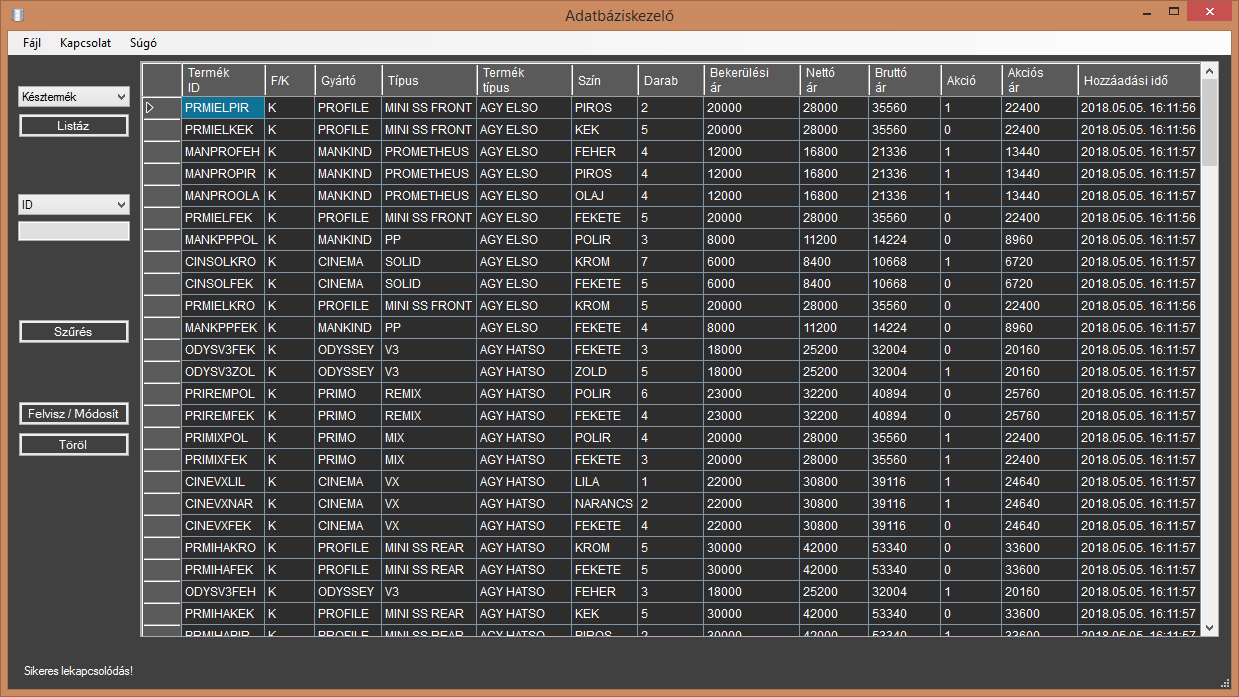
\epsfig{file=kepek/mainForm_afterLogin.png, scale=0.47}
\caption{A főablak (mainForm)} 
\label{fig:mainForm_afterLogin}
\end{figure}

\newpage

\Section{Színek}

A felhasználói felület kialakításakor a könnyű kezelhetőség mellett törekedtem a színeket úgy beállítani, hogy huzamos ideig történő használat esetén is kímélje a szemet, mégis kontrasztos és átlátható maradjon.\par
\setlength{\parindent}{12.5mm}A bejelentkező ablak háttérszíne sötétszürke, az ezen található mezők és gombok alapszínei világosszürkék, a mezőket és a legördülő menüt kitöltő betűszín fekete, egyedül a feliratok fehérek, a jobb kontraszt érdekében. A bejelentkező gomb alapszíne megegyezik a háttérszínnel, valamint az ezen található felirat fehér, ez is a jobb kontraszt érdekében.\par
\setlength{\parindent}{12.5mm}A főprogram háttérszíne megegyezik a bejelentkező ablakéval, a mezők és menük alapszíne világosszürke, és a benne lévő betűszín fekete. A főablakban található adattábla színeinél is törekedtem arra, hogy a szemet kíméljem, mivel elég nagy részt foglal el az ablakból. Ennek színei is sötétszürkék, a cellák hátterei sőtétebbek, míg a fejléc és a sorjelölők világosabb szürkék, a megkülönböztethetőségért. A kijelölés színe kék, mert az a kedvenc színem.





\begin{comment}


%ez itt a dupla kép minta

\begin{figure}[ht]
	\centering
	\begin{minipage}[t]{7cm}
		\centering
		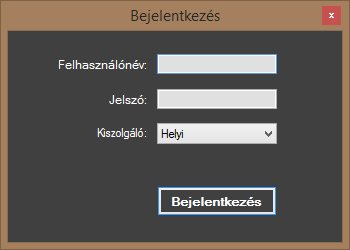
\includegraphics[scale=0.8]{kepek/loginForm_init.png}
		\caption{A bejelentkező ablak inicializáció után (LoginForm)}
		\label{fig:loginForm_init}
	\end{minipage}
	\hspace{0.5cm}
	\begin{minipage}[t]{7cm}
		\centering
		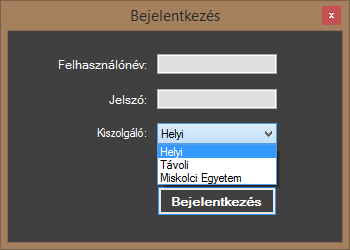
\includegraphics[scale=0.8]{kepek/loginForm_connChoices.png}
		\caption{A bejelentkező ablakban választható kapcsolódási opciók}
		\label{fig:loginForm_connChoices}
	\end{minipage}
 
\end{figure}



%innentol a vecsie
\SubSection{Átlagoló szűrő}

Az átlagoló szűrő segítségével simítani lehet a képet. A képpontok közelebb kerülnek a környezetük átlagához, azaz a kép "simább" lesz, a szűrt kép intenzitásértékei a kiinulási kép intenzitástartományában maradnak. Csökkenti a zajt, de elmossa az éleket igy homályossá teszi a képet.

\example{Itt látható a átlagoló szűrésre egy példa, egy képpont $3 \times 3$-as környezete:
$$
A =
\frac{1}{9} \times
\begin{bmatrix}
54 &26  &32 \\ 
17 &36  &24 \\ 
11 &23  &47 
\end{bmatrix}.
$$
Egyszerű simítási technika, ahol az ablakban lévő intenzitások átlaga az új intenzitás érték: 
$$
\bar{x} =
\frac{54+26+32+17+36+24+11+23+47}{9} =
\frac{270}{9} = 30.
$$}
%Kató tanár úr jegyzet
%wikipédia

\SubSection{Gauss szűrő}

A Gauss szűrő egy bemeneti kép és egy Gauss-kernel konvoluciójával jön létre. Minden egyes képpont értéket a környékének súlyozott átlagaként számolunk úgy, hogy a képpont eredeti értékének a legnagyobb a súlya, míg a távoliak kisebb súlyt kapnak. Ez olyan elmosódást eredményez, amely jobban védi a széleket, mint más egyenletes elmosódási algoritmusok. Egy Gauss függvény felírása egy dimenzióban az alábbi
$$
G(x) =
\frac{1}{\sqrt{2\pi\sigma^{2}}}
\cdot e^{-\frac{x^{2}}{2\sigma^{2}}}.
$$

A Gauss függvény grafikonját \aref{fig:gauss}. ábrán láthatjuk.

% 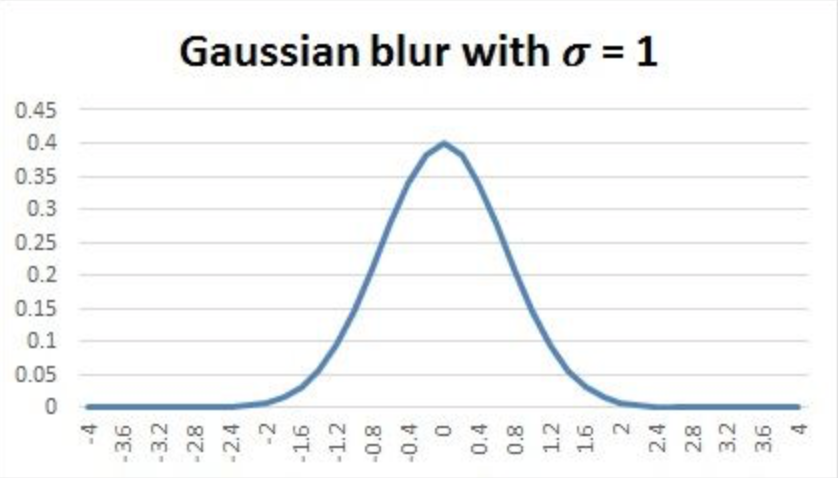
\epsfig{file=kepek/gaussgorbe.png,scale=0.65}

\begin{figure}[h!]
% \centering
\begin{tikzpicture}
\begin{axis}[
    xmin=-4.5,
    xmax=4.5,
    ymin=0,
    ymax=0.45,
    xlabel=$x$,
    ylabel=$G(x)$,
    axis x line=bottom,
    axis y line=left
]
\addplot[mark=none, smooth, blue] {gauss(0, 1)};
\end{axis}
\end{tikzpicture}
\caption{Az egydimenziós Gauss függvény $\mu = 0$ és $\sigma = 1$ paraméterekkel}
\label{fig:gauss}
\end{figure}

Két dimenzióban, két Gauss együttesét kell használni, minden egyes dimenzióban: 
$$
G(x,y) =
\frac{1}{\sqrt{2\pi\sigma^{2}}} \cdot
e^{-\frac{x^{2}+y^{2}}{2\sigma^{2}}},
$$
ahol az $x$ a vízszintes tengely eredetétől való távolság, az $y$ a függőleges tengely eredetétől való távolság, a $\sigma$ pedig a Gauss eloszlás szórása. Két dimenzióban alkalmazva, ez a képlet olyan felületet hoz létre, amelynek körvonalait koncentrikus körök alkotják, a Gauss-eloszlás pedig a középpontból indul.
%wikipédia
%Kató tanár úr jegyzet

\SubSection{Medián szűrő}

Az $a_1, a_2, \dots, a_{2n+1} \in \mathbb{R}$ számok mediánja, a nagyság szerint rendezett számsorozat középső, $(n+1)$-edik eleme. Jelölhetjük például a
$med\{a_1,a_2,\dots,a_{2n+1}\}$ formában.

Teljesül rá az alábbiak:
\begin{itemize}
\item $\min\{a_i\} \leq med\{a_i\} \leq \max\{a_i\}$,
\item $\min\{a_i+c\} = med\{a_i\}+c$,
\item $med\{c\cdot a_i\}=c \cdot med\{a_i\}$.
\end{itemize}

A medián szűrést egy $S \in \mathbb{R}^2$ környezet felett a
$$
J(i,j) = med\left\{I(i+u, j+v) \mid (u, v) \in S \right\}
$$
formában végezhetjük el.

A medián szűrés eredményét az $S$ környezet mérete (és alakja) határozza meg.

\example{Itt látható a medián szűrésre egy példa, egy képpont $3 \times 3$ méretű környezete: $$
M =
\begin{bmatrix}
54 &25  &32 \\ 
17 &37  &22 \\ 
11 &23  &45 
\end{bmatrix}.$$
Nagyság szerint sorba rendezve ezeket az értékeket, úgy hogy  11, 17, 22, 23, 25, 32, 37, 45, 54 akkor a pixel új intenzitása 25 lesz, mivel az a középső érték a sorban.}

%Kató tanár úr jegyzet
\SubSection{Kétoldalú szűrő}

A kétoldalaú szűrő egy nem lineáris, élvédő és zajcsökkentő simító szűrő a képekhez \cite{bilateral}. Az egyes képpontok intenzitását a közeli pixelek intenzitásának súlyozott átlagával helyettesíti. Ez a súly Gauss eloszláson is  alapulhat. Elengedhetetlen, hogy a súlyok nem csak az euklideszi képpontok távolságától, hanem a radiometriai különbségektől is függnek (például tartománykülönbségek, például színintenzitás, mélységi távolság stb.). Ez a kép éles széleit megőrzi. A kétoldalú-szűrő az alábbi alakban írható föl:
\begin{align*}
I^{filtered}(x) &=
\frac{1}{W_p}\sum_{x_i\in\Omega}{I(x_i)f_r(\left \| I(x_i)-I(x) \right \|)g_s(\left \| x_i-x \right \|)}, \\
W_p &=
\sum_{x_i \in \Omega} f_r(\left \| I(x_i)-I(x) \right \|)g_s(\left \| x_i-x \right \|),
\end{align*}
ahol
\begin{itemize}
\item $I^{filtered}$ a filterrel ellátott kép,
\item $I$ az eredeti bemeneti kép,
\item $x$ a koorditánái a jelenlegi pixeleknek amik a szűrőbe kerülnek,
\item $\omega$ az ablak közepe $x$-nek,
\item $f_r$ a tartományi kernel az intenzitások közötti különbségek simítására,
\item $g_s$ a térbeli kernel a koordináták közötti különbségek simítására.
\end{itemize}
A $W_p$ súlyt a térbeli közelség és az intenzitás különbség alkalmazásával határoztuk meg. Vegyünk egy pixelt az $(i, j)$ koordinátákon, amelyet a szomszédos képpontok segítségével kell zajcsökkenteni a képen, és az egyik szomszédos pixele a $(k, l)$ helyen található. Ezután a pixelhez $(k, l)$ hozzárendelt súly az $(i, j)$ pixel zajcsökkentéséhez a következőket adja meg:
$$
w(i, j, k, l) =
\exp \left(
-\frac{(i-k)^{2}+(j-l)^{2}}{2\sigma_{s}^{2}}
-\frac{\left \| I(i,j)-I(k,l) \right \|^{2}}{2\sigma_{r}^{2}}
\right),
$$
ahol $\sigma_s$ és $\sigma_r$ a kiegyenlítési paraméterek, és $I(i, j)$ és $I(k, l)$ a pixelek $(i, j)$ és $(k, l)$ intenzitása.

A súlyok kiszámítása után normalizáljuk őket:
$$
I_{D}(i,j) =
\frac{\sum_{k,l}I(k,l)w(i, j, k, l)}{\sum_{k, l}w(i, j, k, l)},
$$
ahol az $I_D$ a pixel $(i, j)$ zajcsökkentés intenzitása.

A kétoldalú szűrőt két paraméterrel lehet irányítani: $\sigma_r$ és $\sigma_s$. Ezen paraméterek hatását \aref{fig:bilateral}. ábrán láthatjuk.
\begin{itemize}
\item Amikor a $\sigma_r$ paraméter növekszik, a kétoldalas szűrő fokozatosan megközelíti a Gauss konvolúciót, mivel a Gauss-tartomány kiszélesedik és kilapul, ami azt jelenti, hogy a kép intenzitási intervalluma alatt majdnem állandóvá válik.
\item Ahogy a $\sigma_s$ térbeli paraméter nő, a hozzá tartozó nagyobb értékek szerint a kép simább lesz.
\end{itemize}

\begin{figure}[h!]
\centering
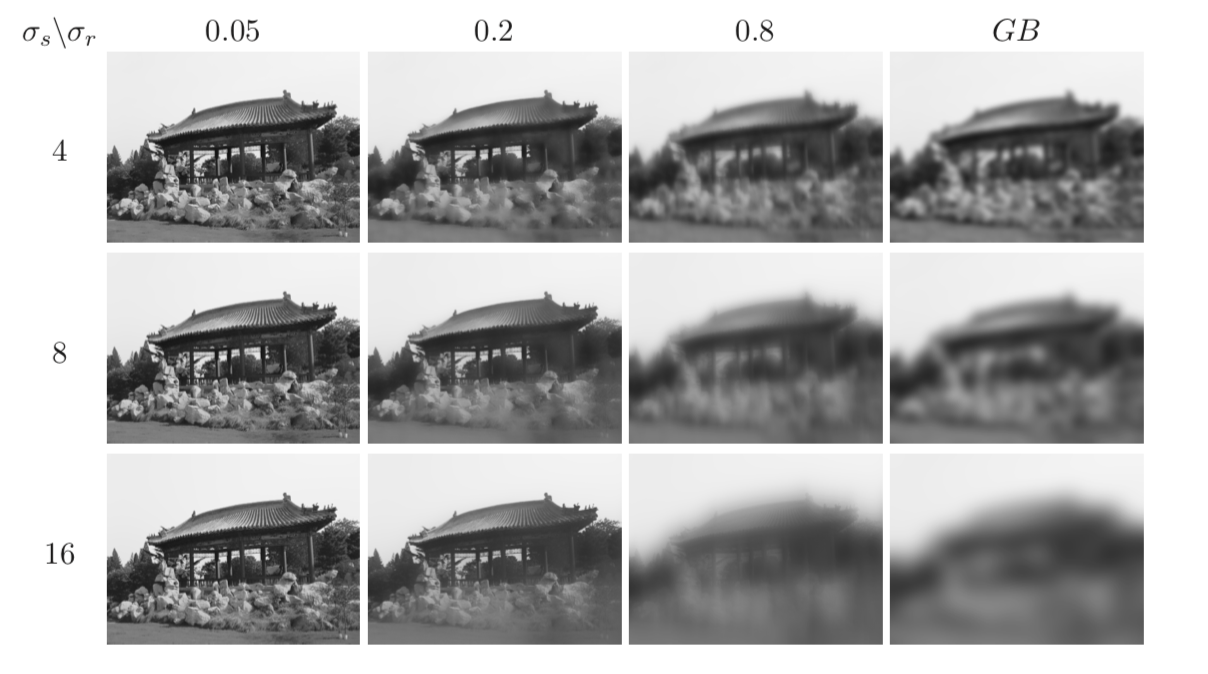
\epsfig{file=kepek/bilateral.png,scale=0.7}
\caption{A $\sigma_r$ és a $\sigma_s$ paraméterek hatása, valamint a Gauss elmosással való összehasonlítás.} 
\label{fig:bilateral}
\end{figure}

\Aref{fig:bilateral1}. ábrán láthatunk egy példát a kétoldalú szűrő elmosására egy bemenetként adott képen, amelyen így az élek megőrzésre kerülnek.

\begin{figure}[h!]
\centering
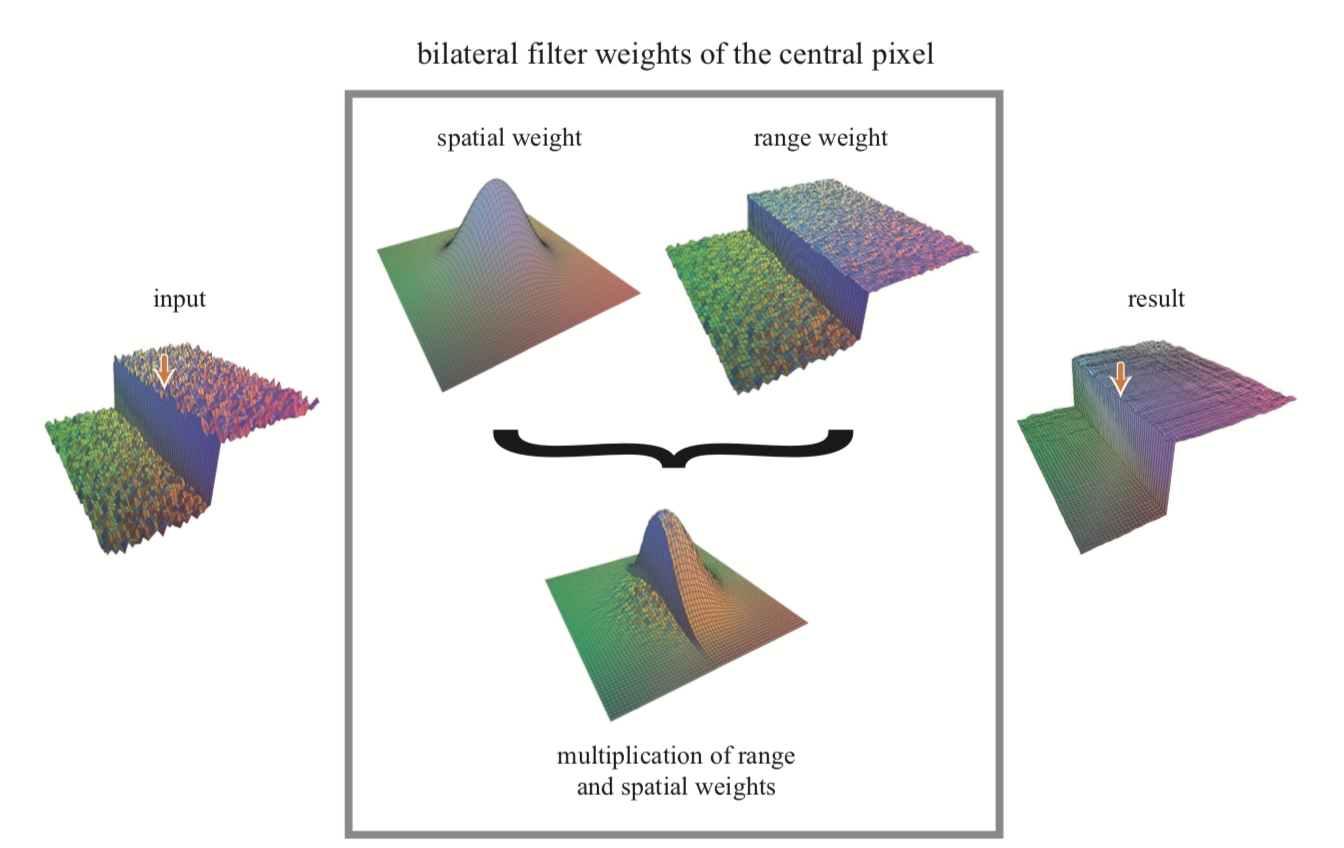
\epsfig{file=kepek/bilateral1.png,scale=0.65}
\caption{A kétoldalú szűrő hatása egy bemeneti képen.} 
\label{fig:bilateral1}
\end{figure}

%wikipédia
%https://people.csail.mit.edu/sparis/bf_course/course_notes.pdf

\newpage

\Section{Éldetektálási módszerek}

Az éldetektálás számos matematikai módszert foglal magába, amelyek olyan pontok azonosítását célozzák meg egy képen, amelyeknél a kép fényereje élesen megváltozik. A kép egy szeletén vizsgálva az intenzitás-profilt jól azonosíthatóak az objektumok határainak megfelelő változások. Az intenzitás-gradiensből következtethetünk az élek helyére és irányára. Jellegzetes élprofilokat láthatunk \aref{fig:elprofilok}. ábrán.

\begin{figure}[h!]
\centering
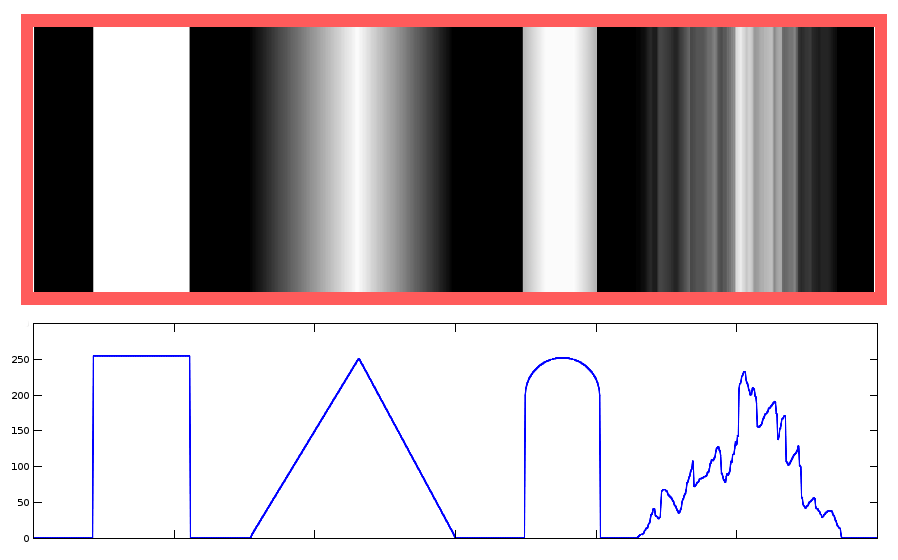
\epsfig{file=kepek/elprofilok.png,scale=0.45}
\caption{Példa tipikus lépcső, tető, vonal és zajos élprofilokra} 
\label{fig:elprofilok}
\end{figure}

A képfüggvény kétváltozós, tehát parciális deriváltakból álló gradiens vektoraink vannak: 
$$
\nabla f =
\left[ \genfrac{}{}{0pt}{}{G_x}{G_y} \right] =
\left[ \frac{\partial f}{\partial x}, \frac{\partial f}{\partial y}  \right]^{T}.$$
A hossza a változás nagyságával egyenlő: 
$$
\left\| \nabla f \right \| =
\sqrt{G_{x}^{2}+G_{y}^{2}} \approx
\left | G_x  \right |+\left | G_y  \right |.
$$
A gradiens a legnagyobb változás irányába mutat: 
$$
\theta = \tan^{-1}\left(\frac{G_y}{G_x}\right).
$$

Digitális képek esetén a pontos, kétváltozós függvényünk nem ismert, ezért a gradiens vektort véges differenciával közelíthetjük:
$$
\frac{\partial f}{\partial x} =
\lim_{\varepsilon \to 0} \left(
\frac{f(x+\varepsilon,y)}{\varepsilon}-\frac{f(x+y)}{\varepsilon}
\right) \approx
\frac{f(x_{n+1}+y)-f(x_n,y)}{\Delta x}.
$$

A gradiens közelítéséhez konvolúciós maszkot is használhatunk.

%Kató tanár úr jegyzet
%wikipédia

\SubSection{Sobel éldetektálás}

A Sobel éldetektáló egy gradiens alapú módszer \cite{sobel}. Ez elsőrendű deriváltakkal működik. A kép első deriváltját külön számítja az $x$ és $y$ tengelyekhez. A deriváltak csak közelítések (mivel a képek nem folytonosak). Ezek közelítéséhez az alábbi kernelt használják a konvolúcióhoz:
$$
G_x =
\begin{bmatrix}
-1&0  &1 \\ 
-2&0  &2 \\ 
-1&0  &1 
\end{bmatrix},
\qquad
G_y =
\begin{bmatrix}
-1&-2  &-1 \\ 
0&0  &0 \\ 
1&2  &1 
\end{bmatrix}.
$$
Az első mátrix a vízszintes, a második mátrix a függőleges kernel. A bal oldali kernel megközelíti a deriváltat az $x$ tengely mentén, a jobb oldali pedig az $y$ tengely mentén. Ezen információk felhasználásával számíthatjuk ki az alábbiakat:
\begin{itemize}
\item magnitudója vagy "erőssége" az élnek: $\sqrt{G_{x}^{2}+G_{y}^{2}}$,
\item megközelítő erősség: $ \left\| G_x \right \| + \left\| G_y \right \|$,
\item az él iránya: $arctan\left(\frac{G_y}{G_x}\right)$.
\end{itemize}

%Kató tanár úr jegyzet
%http://aishack.in/tutorials/sobel-laplacian-edge-detectors/

\SubSection{Laplace éldetektálás}

A Laplace éldetektáló csak egy kernelt használ \cite{sobel}. Másodfoku deriváltakat számol ki egy lépésben. Itt van néhány elterjedt kernel:
$$
G_1 =
\begin{bmatrix}
 0 & -1  & 0 \\ 
-1 &  4  &-1 \\ 
 0 & -1  & 0 
\end{bmatrix} 
\qquad
G_2 =
\begin{bmatrix}
-1 & -1 & -1 \\ 
-1 &  8 & -1 \\ 
-1 & -1 & -1 
\end{bmatrix}
$$
Az első mátrix a laplace operátor, a második mátrix a laplace operátor átlókkal.

Használhatjuk akár csak az egyiket, vagy ha jobb közelítést szeretnénk, létrehozhatunk egy 5x5-ös kernelt (aminek a középpontja 24, és minden más -1).

Egy komoly hátrány azonban van, mivel másodfokú deriváltakkal dolgozunk, a laplace éldetektáló rendkívül érzékeny a zajokra. Általában zajcsökkentés szükséges. Néhány fontos további jellemzője:
\begin{itemize}
\item elmosódott élek esetén pontosabb lokalizálást érhetünk el,
\item ebben az esetben csak az élek helyét tudjuk meghatározni, az irányát nem,
\item az operátor nem érzékeny az elforgatásra.
\end{itemize}

%Kató tanár úr jegyzet
%http://aishack.in/tutorials/sobel-laplacian-edge-detectors/

\SubSection{Canny éldetektálás}

Az Canny éldetektálás olyan technika, amely a különböző objektumokból származó hasznos strukturális információkat kivonja, és drasztikusan csökkenti a feldolgozandó adatok mennyiségét. Számos számítógépes képfeldolgozó rendszerben széles körben alkalmazzák. Canny úgy találta, hogy viszonylag hasonlóak a különféle éldetektálás alkalmazására vonatkozó követelmények. Így a követelményeknek megfelelő éldetektáló megoldás számos helyzetben megvalósítható. 
\\ \\
\textbf{Algoritmus:}\\ \\
\indent 1. Gauss simítás\\
\indent 2. A kép intenzitás gradiensének megkeresése\\
\indent 3. Nem-maximumok elhagyása\\
\indent 4. Hiszterézis küszöbölés \\ 

\subsubsection{1. Gauss simítás}

Mivel az éldetektálás eredményeit a képzaj is könnyen befolyásolja, elengedhetetlen a zaj kiszűrése, hogy megelőzze a zaj által okozott hamis detektálást. A kép simítása érdekében Gauss szűrőt alkalmazunk. Ez a lépés enyhén simítja a képet, hogy csökkentse a nyilvánvaló zaj hatását a éldetektálásra.

\subsubsection{2. A kép intenzitás gradiensének megkeresése}

A kép élei különböző irányokban jelennek meg, így a Canny algoritmus négy szűrőt használ a vízszintes, függőleges és átlós élek detektálásához az elmosódott képen. Éldetektáló operátor (például Sobel) az első derivált értékét vízszintes irányban $(G_x)$ és a függőleges irányba $(G_y)$ adja vissza. Ebből meghatározható az él-gradiens és az irány:
$$
G = \sqrt{G_{x}^{2}+G_{y}^{2}},
\quad
\Theta = arctan2\left(\frac{G_y}{G_x}\right).
$$
ahol $G$ a hypot függvény segítségével számítható ki, és az arctan2 az arctangens függvény két argumentummal.

Az élirány-szög négy függőleges, vízszintes és két átlós (0 , 45 , 90  és 135 fokok) függőleges szögek egyikére kerekítve van. Az egyes színsávokba eső élek iránya meghatározott szögértékekre van beállítva.

\subsubsection{3. Nem-maximumok elhagyása}

A nem-maximumok elhagyása a "vékony" élekre alkalmazzák. A gradiens kiszámítása után a gradiens értékből kivont él még mindig homályos. A 3. kritérium vonatkozásában csak egy pontos válasz lehet az élre. Így a nem-maximumok elhagyása segíthet elhagyni a gradiens értékeket (0-ra állítva), kivéve a lokális maximumokat, amelyek a legerősebb intenzitásérték-változást jelzik. Az algoritmus a következő, minden pixelre a gradiens képen:
\begin{itemize}
\item Hasonlítsa össze az aktuális képpont él-erősségét a pixel él-erősségével, pozitív és negatív gradiens irányba.
\item Ha az aktuális képpont él-erőssége a legnagyobb az azonos irányú maszk más képpontjaihoz képest, az érték megmarad. Ellenkező esetben az érték elhagyásra kerül.
\end{itemize}

Bizonyos implementációkban az algoritmus a folyamatos gradiens irányokat különálló diszkrét irányokba sorolja, majd egy $3 \times 3$ szűrőt rak az előző lépés kimenetre. Minden pixelben elhagyja a középső képpont él-erősségét (az értékét 0-ra állítva), ha nagysága nem nagyobb, mint a két szomszéd nagysága a gradiens irányba.

\subsubsection{4. Hiszterézis küszöbölés}

Eddig az erős élű képpontokat minden bizonnyal be kell vonni a végső élbe, mivel ezek a kép valódi éleiből származnak.Vannak azonban viták a gyenge élű képpontokról, mivel ezek a pixelek kiválaszthatók az igazi élről, vagy a zaj/színváltozatokról. Pontos eredmény elérése érdekében az utóbbi okok által okozott gyenge éleket el kell távolítani. Általában gyenge él pixeleket okoznak, az igazi élek amikor erős élű pixelekhez kapcsolódnak, amíg a zajok nem kapcsolódnak hozzá. Az élkapcsolat nyomon követéséhez a blob elemzést kell végre hajtani, ami egy gyenge élű pixel és 8-as kapcsolatú szomszédos pixelek figyelembevétele. Mindaddig, amíg van egy erős élű pixel, amely részt vesz a blob elemzésben, a gyenge élű pontot lehet azonosítani, amit meg is kell őrizni.

%Kató tanár úr jegyzet
%wikipédia

\Section{Szegmentálás}

Számítógépes látásmódban a képszegmentálás a digitális kép több szegmensbe való felosztása. A szegmentálás célja egyszerűsíteni és/vagy megváltoztatni a kép reprezentációját ezzel könnyebbé téve a kép elemzését. A kép szegmentálását általában objektumok és határok megtalálásához használják. Pontosabban, a képszegmentálás egy címke hozzárendelését jelenti a kép minden képpontjához úgy, hogy az azonos címkével rendelkező pixelek bizonyos tulajdonságokkal rendelkeznek. A képszegmentáció eredménye olyan szegmensek csoportja, amelyek együttesen fedik le a teljes képet vagy a képből kinyert kontúrt. Valamennyi régióban lévő pixelek hasonlóak bizonyos jellemzők vagy számított tulajdonságok, például szín, intenzitás vagy textúra tekintetében. A szomszédos régiók szignifikánsan különböznek az azonos jellegzetességek tekintetében.

%wikipédia

\SubSection{Mean shift algoritmus}

Mean shift egy eljárás a maximális értékek azonosítására, ahol a sűrűségfüggvény módjait a funkciótól vett diszkrét adat szolgáltatja. Ez egy iteratív módszer, az $x$ kezdeti becslésével kezdünk. Adjuk meg a $K(x_i - x)$ kernel függvényt. Ez a függvény határozza meg a közeli pontok súlyát az átlag újraértékeléséhez. Általában egy Gauss kernelt használunk az aktuális becsléshez képest, $K (x_i - x) = e ^ {- c || x_i - x || ^ 2}$. A $K$ által meghatározott ablak sűrűségének súlyozott átlaga: 
$$
m(x) =
\frac{\sum_{x_i \in N(x)}K(x_i-x)x_i}{\sum_{x_i \in N(x)}K(x_i-x)},
$$
ahol $N(x)$ az $x$ szomszédsága, olyan pontok halmaza, amelyekhez $K(x_ {i}) \neq 0$.

Az $m (x) -x$ különbséget az Fukunaga és a Hostetler átlagos eltolódásának nevezik. Az mean shift algoritmus most beállítja az $x \leftarrow m(x)$ értéket, és megismétli a becslést, amíg $m(x)$-ig konvergál.

\Section{Küszöbölés}

% TODO: Érdemes lehet még az éldetektálás elé rakni!

A küszöbérték a képszegmentálás legegyszerűbb módja. A szürkeárnyalatos képből küszöbérték használatával bináris képek készíthető. Tételezzük fel, hogy az objektum és a háttér eltérő intenzitású, vagyis nagy a kontraszt. Az objektum és a háttér önmagában homogén intenzitású. A küszöbölést így a hisztogram alapján választott megfelelő értékkel el tudjuk végezni (\ref{fig:threshold}. ábra).

Zajos kép esetén nehéz kielégítő köszöbértéket meghatározni, tehát a szegmentálás inhomogén lesz, erre a zajszűrés jelenthet megoldást.

%wikipédia

\begin{figure}[ht]
\centering
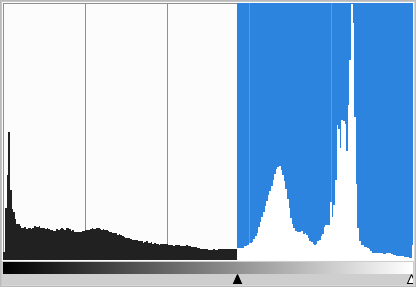
\epsfig{file=kepek/threshold.png,scale=0.65}
\caption{Példa a hisztogram alapján egy megfelelő küszöbérték megválasztására} 
\label{fig:threshold}
\end{figure}

% TODO: Az alábbit még át kell majd kicsit fogalmazni!

\example{Sötét objektum világos háttérben:\\
$f(x,y)$- bemeneti kép;\\
$t(x,y)$- szegmentált kép;\\
$T$=küszöbérték\\
\\
$f(x,y)\leq T$, akkor $t(x,y)=1$, azaz objektum.\\
$f(x,y)> T$, akkor $t(x,y)=0$, azaz háttér.
}\\\\
Léteznek adaptív eljárások, melyek az input képhez automatikusan választják ki az optimális küszöbértéket. Ebből vannak globális és lokális küszöbértéket meghatározó algoritmusok. A globális köszöbölésre alkalmas algoritmusok hisztogramból klaszterezéssel számított értékekel dolgoznak. Ilyen például az Isodata valamint az Otsu algoritmus. A lokális küszöbölés változó értékekkel dolgozik, például egyenletlen megvilágítás. Amennyiben az objektum és a háttér kontrasztja globális küszöbölés után, lokálisan még mindig nagy, akkor alkalmazzuk a lokális küszöbölést, például Niblack algoritmust.

%Kató tanár úr jegyzet
%wikipédia

\SubSection{Izodata algoritmus (Yanni)}

Jól használható, ha az előtér és a háttér körülbelül ugyanannyi képpontból áll. Az algoritmus az alábbi lépésekből áll.
\begin{itemize}
\item[1.] Inicializálás: a hisztogramot kétrészre osztjuk, célszerűen a felezőponton: $T_0$
\item[2.] Kiszámítjuk az objektum valamint a háttér intenzitásának a középértékét: $M_i, m_i$
\item[3.] Az új küszöbérték a két középérték átlaga: $T_i=(M_i+m_i)/2$
\item[4.] Vége ha a küszöbérték már nem változik: $T_k+1=T_k$
\end{itemize}

%Kató tanár úr jegyzet

\SubSection{Otsu algoritmus}

A bemeneti kép $L$ szürkeárnyalatot tartalmaz, a normalizált hisztogram minden $x$ szürkeértékéhez megadja az előfordulási gyakoriságát, vagyis a valószínűségét: $p_x$. Keressük azt a $T$ küszöbszámot, amely maximalizálja az objektum-háttér közötti varianciát.

\textbf{Az előtér/háttér pixelek gyakorisága és középértéke:}

Háttér valószínűsége:
$$
B(T) = \sum\limits_{x=1}\limits^{T}p_x 
$$

Objektum valószínűsége:
$$
1-B(T)=\sum\limits_{x=T+1}\limits^{L}p_x
$$

Legyen $m(T)\equiv \sum\limits_{x=1}\limits^{T}xp_x$, a teljes kép középértéke: $\mu \equiv m(L) = \sum\limits_{x=1}\limits^{L}xp_x$,

Háttér középértéke:
$$
\mu_B =\frac{m(T)}{B(T)}
$$

Objektum középértéke:
$$
\mu_O =\frac{\mu-m(T)}{1-B(T)}\\
$$

\textbf{Az előtér/háttér pixelek szórása:}

$$
\sigma^2_B =
\frac{1}{B(T)}\sum\limits_{x=1}\limits^{T}(x-\mu_B)^2 p_x,
$$
$$
\sigma^2_O =
\frac{1}{1-B(T)}\sum\limits_{x=T+1}\limits^{L}(x-\mu_O)^2 p_x
$$

\textbf{A teljes kép szórása:}
$$
\sigma^2 =
\sum_{x=1}^T(x-\mu)^2 p_x + \sum_{x=T+1}^L(x-\mu)^2 p_x =
\dots =
$$
$$
= B(T)\sigma_B^2+(1-B(T))\sigma_O^2 + (\mu_B-\mu)^2B(T)+(\mu_O-\mu)^2(1-B(T)) \equiv \sigma^2_W(T)+\sigma^2_C(T)
$$
ahol, a $B(T)\sigma_B^2+(1-B(T))\sigma_O^2 = \sigma^2_W(T)$, osztályon belüli varianciától függ és a $(\mu_B-\mu)^2B(T)+(\mu_O-\mu)^2(1-B(T)) = \sigma^2_C(T)$, osztályokközötti varianciától függ. A $\sigma^2$ konstans, és $T$-t úgy kell beállítani, hogy $\sigma_C^2(T)$ a lehető legnagyobb legyen:
$$
\sigma^2_C(T) = \dots = \frac{(\mu(T)-\mu B(T))^2}{B(T)(1-B(T))}
$$
A hisztogram elejéről kezdve nézzük meg minden szürkeértéket, mint lehetséges küszöböt. Kiszámoljuk a $\sigma^2_C(T)$ értéket a $\mu(T)$ és $B(T)$  segítségével, mindaddig növeljök a $T$ értékét, amíg $\sigma^2_C(T)$ kövekszik. Ez az algoritmus feltételezi, hogy $\sigma^2_C(T)$-nek egy maximuma van.

%Kató tanár úr jegyzet

\SubSection{Niblack algoritmus}

Egyetlen küszöb nem elegendő az objektum és a háttér szétválasztásához. Ezért változó köszöbérték $(T(i,j))$ kell, amely követi az intenzitás változásokat:
$$
T(i,j)=\mu(i, j) + k \sigma(i, j)
$$
Az $(i,j)$ adott környezetében, $\mu(i,j)$ a középértéket jelenti, $\sigma(i, j)$ pedig a szórást. A $k$ egy súly, ami megmutatja mennyire vegyük figyelembe a szórást.

Ha $k < 0$, akkor sötét az objektum,
Ha $k > 0$, akkor világos az objektum.

A globális és a lokálisan változó küszöbértékre láthatunk egy-egy szemléltetést \aref{fig:const_thresh}. és \aref{fig:adaptive_thresh}. ábrákon.

\begin{figure}
\centering
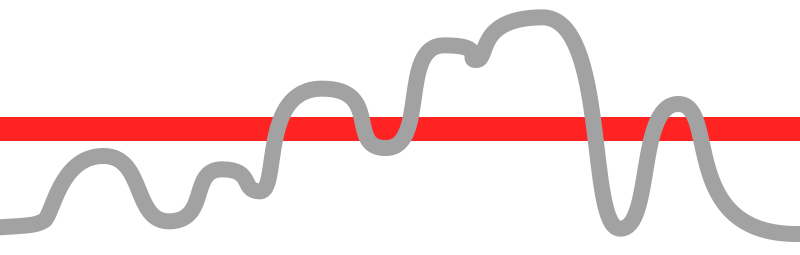
\includegraphics[scale=0.5]{kepek/const_thresh.png}
\caption{Intenzitásértékek küszöbölése globális küszöbérték mellett}
\label{fig:const_thresh}
\end{figure}

\begin{figure}
\centering
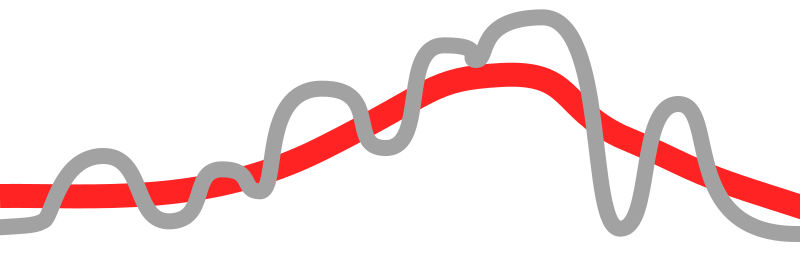
\includegraphics[scale=0.5]{kepek/adaptive_thresh.png}
\caption{Intenzitásértékek küszöbölése lokális/adaptív küszöbértékkel}
\label{fig:adaptive_thresh}
\end{figure}

%Kató tanár úr jegyzet

\end{comment}
% !TEX encoding = UTF-8 Unicode

\Chapter{Adatbázis kapcsolat}


\setlength{\parindent}{12.5mm}Az Oracle Database Express Edition adatkapcsolat szempontból két fő komponensből áll, az egyik a szerver, a másik a kliens. Ez egy hierarchiailag alárandelt kapcsolat, a kliens kapcsolódik a szerverhez, adatokat kér, amiket a szerver feldolgoz és - ha a kliens megfelelő jogosultsággal rendelkezik - kiszolgál. A megfelelő működéshez egy szervernek futnia kell, amihez kapcsolódhat(nak) a kliens(ek). A szerver és kliens települhet ugyan azon eszközre (sőt, egyszerre lehet telepítve 32 és 64 bites verzió is, ami több esetben javasolt is), valamint futásuk is történhet egy időben és egy számítógépen, így a kis infrastruktúrával és alacsony költségvetéssel rendelkező vállalkozásoknak is megfelelő megoldás lehet. A több klienst használó vállalatok pedig jellemzően egy külön erre dedikált szerverhez kapcsolódnak, és arra nem is kötelező az adatbázis kezelő szoftver telepítése, mert az Oracle beépített adminisztrációs felületéről (rendelkezik grafikus felhasználói felülettel és parancssorral is) a legtöbb szükséges teendőt el lehet végezni, ám a szervert érintő rendszerbeállítások kizárólag parancssoron keresztül érhetőek és vegezhetők el.

\Section{Kapcsolatok típusai}

\SubSection{Helyi kapcsolat}
	\label{helyi_kapcsolat}

Amennyiben a szerver és a kliens egy számítógépen fut, a kapcsolat típusa \textit{Helyi kapcsolat}, tehát a klienssel egy lokális kiszolgálóhoz kapcsolódunk. Ilyen esetekben - bár egy eszközön futnak - a kliens és a szerver logikailag elkülönül egymástól, viszont a hálózati címzés a helyi hálózaton át valósul meg, tehát az elérés történhet a 127.0.0.1 IP címen, vagy a localhost néven keresztül. Ez hasznos lehet több klienst használó vállalat esetén, ahol a kliens gépek a lerakatokban, vagy külső raktárokban találhatóak, de a központi raktárban vagy szerverszobában található fő szervergépről is elérhető és menedzselhető az adatbázis.\par
\setlength{\parindent}{12.5mm}Bizonyos esetekben fennálhat a vállalat kérése, hogy csak a helyi kapcsolatot használó számítógépről legyen elérhető a napló tábla, ami a beépített eszközzel is elérhető, de célszerű ilyenkor is az alkalmazást használni, a már megszokott kezelőfelület miatt. Ez néhány soros módosítás után könnyen megvalósítható, így a kliens és szervergépeken futó programok már külön instanciák.

\SubSection{Távoli kapcsolat}
	\label{tavoli_kapcsolat}

Távoli kapcsolat esetén a felhasználónak lehetősége van egy általa meghatározott kiszolgálóhoz kapcsolódni, ehhez szüksége van az adott szerver IP címére, portjára és a rajta futó adatbázis verziójának megnevezésére. Ennek formálisan is meg kell felelnie, de a szintaktikához segítséget nyújt a bejelentkező ablakon található információs ikon. Alkalmas kliens gépek esetén külső raktárakból történő hozzáférésre, valamint adott szerver elérésére bárhonnan, amennyiben a szerver és a kliens online, az átjáráshoz használt port nincs blokkolva a tűzfal által, továbbá a felhasználó rendelkezik érvényes hozzáféréssel az adatbázishoz.\par
\setlength{\parindent}{12.5mm}Amennyiben az előző pontban említett kérés fennáll a vállalat részéről, úgy a csak távoli kapcsolattal rendelkező instanciák jellemzően nem kapnak jogot arra, hogy a napló táblát lássák. A napló tábla egyébként is alacsony szinten védett, de így információhoz sem juthatnak azok, akiknek egyébként sem lenne hozzá jogosultságuk.
\vskip 0.5cm
A távoli kapcsolat kézi beállításához segítség a következő, \ref{miskolci_egyetem_kapcsolat} pontban.


\SubSection {Miskolci Egyetem}
	\label{miskolci_egyetem_kapcsolat}
Ez az opció a szoftver megjelenésének és működésének bemutatásához készült. Ebben az esetben a szoftver a Miskolci Egyetem Általános Informatikai Intézeti Tanszékén található Oracle szerveréhez kapcsolódik, ez a kapcsolat jellemzően a tanulmányi időszakokban érhető el, akkor megbízhatóan működik. Az alkalmazás, az információ- és adatátvitel, valamint a hozzá tartozó kapcsolat megfelelően tesztelhető rajta.
Az ehhez tartozó belépési adatok:\par

Mivel ez is egy távoli elérés (a külön listázás csak a kényelmesebb használat érdekében történt), ugyan ez az adatkapcsolat kipróbálható a \textit{Távoli} opció használatával is, a belépéshez szükséges adatok, valamint az egyetemi Oracle adatbázis szerver elérhetősége: 

\begin{center}
\begin{tabular}{rl}
Felhasználónév: & \textit{\textbf{duritt}}\\
Jelszó: & \textit{\textbf{t6716g}}\\
Cím: & \texttt{193.6.5.58:1521/XE}
\end{tabular}
\end{center}

\par

Az adatbázis, amelyhez a szoftver ezen a kapcsolatul keresztül kapcsolódik elérhető a Miskolci Egyetem által a tanulmányi időszakban biztosított szerver APEX felületén is, ahol grafikusan és parancsokkal is módosíthatjuk az adatbázis tartlmát, valamint lekérdezéseket, kimutatásokat, metaadatokat is lekérhetünk, emelett web-es alkalmazást is generálhatunk ezen keresztül. Ennek elérése:

%ezt ellenőrizni!
<<ellenorizni>>

\begin{center}
\begin{tabular}{rl}
Cím: & \texttt{193.6.5.58:8080/apex}\\
Munkaterület: & \textit{\textbf{duritt}}\\
Felhasználónév: & \textit{\textbf{admin}}\\
Jelszó: & \textit{\textbf{t6716g}}\\

\end{tabular}
\end{center}

\Section{Adatkapcsolat felépítése}
Az Oracle adatbázis-kapcsolat felépítésénél az elnevezések tetszés szerintiek lehetnek, de célszerűek a beszédes nevek, hogy közben, vagy esetleg a későbbiekben a kód a fejlesztő számára átlátható legyen \textit{(kivételt képeznek ezalól a nagy költségvetésű fejlesztést igénylő szoftverek, amelyeknél a cél a visszafejtés lehető legnehezebbé tétele)}, felépítés szerint:

\begin{itemize}

	\item \texttt{OracleConnection con;}
		\\Egy \texttt{OracleConnection} típusú objektum, ami valójában egy kapcsolatleíró string, mely az Oracle adatbázisokkal való kapcsolatot kezeli.

	\item \texttt{DataSet ds = new DataSet();}
		\\A \texttt{DataSet} példányosítása a lekérdezett adatok adattáblában történő tárolásához.
		\\Ez egy adatbázis a memóriában, amelynek szerepe, hogy az adattábla osztályban létrehozott objektumokat tárolja.

	\item \texttt{DataTable dt = new DataTable();}
		\\Az adattábla (\texttt{DataTable}) objektum \texttt{dt} példánya egy logikai táblát hoz létre a memóriában az adatbázis-szerverről áthozott adatok alapján.Amikor ez megtörténik, a program közvetlenül innen olvas majd, és a felhasználó által létrehozott módosítások is itt tárolódnak. Ennek tartalma lehet:
		\begin{itemize}
		\item \textit{Táblák:} Logikailag összetartozó értékek halmaza, elrendezése sorokban és oszlopokban történik.
		\item \textit{Mezők}: Cellák, melyekbe az adott cella típustáól függően adatot vihetünk be. Itt értékellenőrzés történik, azaz egy szám típusú cellába nem írhatunk karaktersorozatot.
		\item \textit{Sorok:} Jellemzően egy adott rekordhoz kapcsolódó értékek sorozata, a logikai szeparálást segítve külön cellákba rendezve, így a sorban lévő mezők alkoltnak oszlopokat.
		\item \textit{Oszlopok:} Az említett elrendezés függőlegesen összetartozó elemei, például telefonszámok egymás alatt. Létezhetnek oszlopok, amelyek elemeinek különbözőeknek kell lenniük, jellemzően ezek az elsődleges kucslok, egyedi azonosítók (ID).
		\item \textit{Nézetek:} Lekérdezés vagy több tábla kiválasztott oszlopai egymás mellett. Használatuk olyan esetekben történik, amikor több táblából szeretnénk adatokat egymás mellett úgy látni, hogy egy új nézőpontból közelíthessük meg a vizsgált tartalmat.
		\item \textit{Indexek:} A táblában lévő keresés felgyorsítására alkalmazott eszköz, jellemzően nagy méretű adatbázisokban használják, megvalósításai: hash-kód vagy bináris fa. Az optimalizálás és a megfelelően alkalmazott indexelés a nagy méretű adatbázisokban a futási időt $\mathcal{O}(n)$ -ről $\mathcal{O}(\log{}n)$-re csökkenti. Ez azt jelenti, hogy a nem megfelelően indexelt adatbázisok lineáris (az elemek számával egyenes arányban lévő) futási idejűek, tehát a az elemszámok növekedésével a futási idő is azonos mértékben nő, így ha az elemszám a duplájára nő, a futási idő is megduplázódik. A megfelelően indexelt adatbázisok esetén a futási idő logaritmikus, ami gyakorlatilag konstansnak vehető a logaritmus függvény miatt.
		\item\textit{ Kényszerek:} A kényszerek a táblákra és az abban szereplő oszlopokra vonatkozó, a megfelelő működés, konzisztencia biztosítását szolgáló szabályok. Több felhasználós környezetben a párhuzamos hozzáférés miatt problémás lehet, például ha egy időben szeretnének létrehozni megegyező azonosítójú terméket. Szintaktikailag a DDL része.
		\item \textit{Kapcsolatok:} Ahogy a relációs adatbázis elnevezés is utal rá, ezen adatbázis működésének alapja a táblák, mezők és értékeik közti kapcsolat, így ezeket is tárolni kell.
		\item \textit{Metaadatok:} Adatok az adatokról, amelyek a hatékonyság, integritásőrzés, adatvédelem biztosítását szolgálják.		
		\end{itemize}

	\item \texttt{OracleDataAdapter da = new OracleDataAdapter();}
		\\Ez az összekötő kapocs a fizikai adathalmaz és a memóriában tárolt, strukturált adathalmazok között.

	\item \texttt{OracleCommandBuilder builder = null;}
		\\Egy nem örökölhető osztály, amely automatikusan generálja azokat a parancsokat, amelyekkel a felhasználó által, futásidőben történő adatmódosításokat összeegyezteti a \texttt{DataSet}-ben lévő értékekkel.
	
	\item \texttt{OracleCommand cmd = new OracleCommand();}
		\\Az ehhez kapcsolódó átadott paraméterekkel (commandText (a lekérdezés szövege), \texttt{OracleConnection conString} (a kapcsolódást biztosító string)) egy új példányt hoz létre az \texttt{OracleCommand} osztályon belül, amellyel a lekérdezést majd végrehajtja.

	\item \texttt{string conString = String.Format("User Id=\{0\};Password=\{1\};" + "Data Source=\{2\};Pooling=false;", input\_uid, input\_pw, server\_address);}
		\\Ez a kapcsolódást biztosító string, azaz karaktersorozat.
		\\Jelen esetben egy formázott stringről van szó, mert az azonosító, jelszó és az adatforrás értékei a felhasználó általi input alapján kerülnek átadásra, de lehet előre definiált, statikus érték is. Erről bővebben a \ref{adatkapcsolat_parameterezese} szekcióban.

	\item \texttt{con = new OracleConnection(conString);}
		\\Ez az \texttt{Oracle} osztályon belül létező\textit{Connection} típus, ami az adatbázis eléréséért felel. Használatakor egy új példány jön létre az osztályban. Ez metódusként használható, így a zárójelben átadott \texttt{conString}-gel a kapcsolódáshoz szükséges adatok is átadásra kerülnek. Ennek értékei kerülnek átadásra a már létrehozott \texttt{con} változóba, és a későbbiekben ennek használatával jön létre a közvetlen adatkapcsolat.

	\item \texttt{con.Open();}
		\\Ha a példányosított \texttt{OracleConnection} megfelelő adatokkal rendelkezik, a \texttt{.Open()} metódus létrehozza a kapcsolatot a kliens és a szerver között. Amennyiben nincsenek megfelelő adatok, a metódus akkor is lefut, de a kapcsolódás sikertelen lesz.

\end{itemize}

\Section{Adatkapcsolat paraméterezése}
\label{adatkapcsolat_parameterezese}
A bejelentkező ablakon keresztüli bejelentkezéskor a kapcsolatot és az adatbázishoz való hozzáférés érvényességét maga az adatbázis-szerver ellenőrzi. A LoginFormba beírt felhasználónév és jelszó, valamint a manuális kapcsolódás esetén a kézzel beírt elérési cím (a helyinél és a távolinál is létezik cím, de ez a minidig ugyan az, így nem szükséges sem kézzel beírni, sem megjeleníteni) egy a kapcsolat felépítéséhez elengedhetetlen, a kapcsolódáshoz tartozó azonosítási és kapcsolódási adatokat tartalmazó stringbe (connectionString) kerül, így minidig a bejelentkező ablakba írt érték és a választott kapcsolat alapján, dinamikusan kap értéket.
\par
A paraméterátadás megvalósítása a forráskódban:

\begin{cpp}
string conString = String.Format(
		   "User Id={0};Password={1};" +
		   "Data Source={2};Pooling=false;",
		   input_uid, input_pw, server_address);
\end{cpp}

ahol:
\begin{itemize}
	\item{\itshape \{0\}} a felhasználónév (minden esetben a mezőbe írt érték adódik át),
	\item{\itshape \{1\}} a jelszó (minden esetben a mezőbe írt érték adódik át),
	\item{\itshape \{2\}} az adatkapcsolat címe (itt csak akkor adódik át a mezőbe írt érték, ha a listából a \textit{Távoli} van kiválasztva, egyébként választástól függően (\textit{Helyi} vagy \textit{Miskolci Egyetem}) előre definiált értékek adódnak át).
\end{itemize}

Ha az alkalmazást megrendelő fél nem szeretne a szoftverbe beléptető funkciót (ami nem javasolt, de a védelem megoldható különböző operációs rendszerbeli mechanizmusokkal, harmadik fél által készített szoftverekkel, vagy akár az eszköz teljes izolálásával, ugyanis a lokális szerveren futó adatbázishoz nem szükséges aktív internetkapcsolat), abban az esetben a connectionString felépítésének és tartalmának nem szükséges dinamikusnak lennie, statikus módon is megoldható:

\begin{cpp}
string conString = "User Id=Vallalat001;Password=Jelszo123;" +
                   "Data Source=127.0.0.1:1521/XE;Pooling=false;";
\end{cpp}

ahol:
\begin{itemize}
	\item a felhasználónév: \texttt{Vallalat001}
	\item a jelszó: \texttt{Jelszo123}
	\item az adatforrás: \texttt{127.0.0.1:1521/XE}, amiből:
	\begin{itemize}
		\item a szerver IP címe: \texttt{127.0.0.1}
		\item a port: \texttt{1521}
		\item az adatbázispéldány neve (SID): \texttt{XE}
	\end{itemize}
\end{itemize}



\begin{comment}

%innentol vecsie

\Section{Cartoon-style filter}

Az első filter egy rajzfilm jellegű (\textit{cartoon-style}) filter, amely az éleket kiemeli és a színeket elmossa. A szűrőhöz az ötletet Michael Beyeler hasonló szűrője adta, melyet Python nyelven készített el \cite{beyeler}.

A műveletekhez Gauss-piramist, kétoldalú szűrést, medián szűrést, illetve adaptív küszöbölést használtam. A szűrés eredményére egy példát \aref{fig:cartoon1}. ábrán láthatunk.

\begin{figure}[ht]
\centering
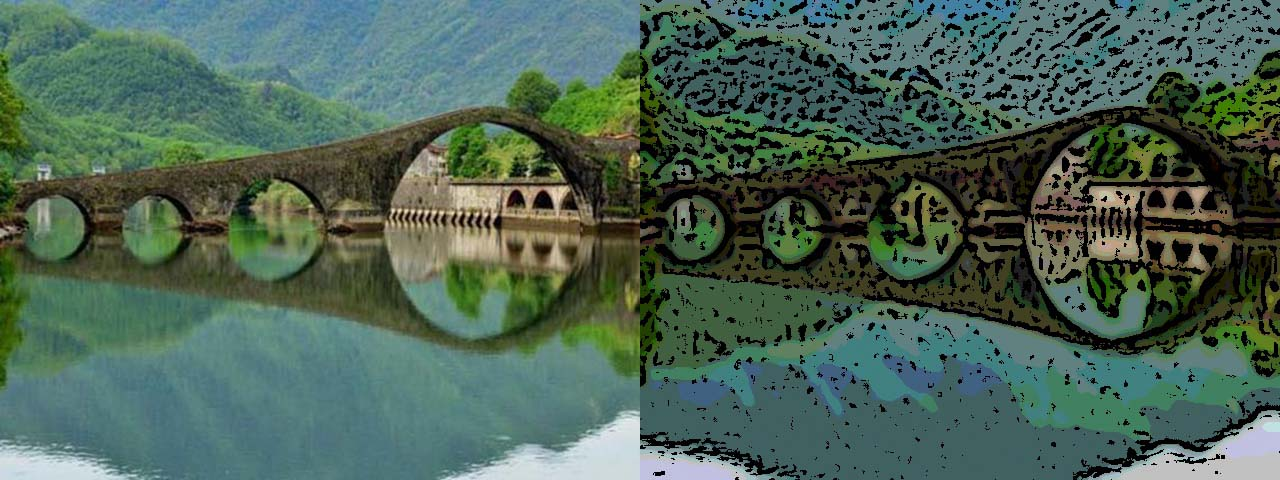
\epsfig{file=kepek/1_cartoon_filter.jpg, width=15cm, height=5.625cm}
\caption{Bal oldalon az eredeti-, jobb oldalon pedig a filterrel ellátott kép látható (forrás: \textit{http://www.erdekesvilag.hu/elkepeszto-tajkepek/})} 
\label{fig:cartoon1}
\end{figure}

\SubSection{Gauss-piramis és kétoldalú szűrő}

Első lépésben az eredeti képet lekicsinyítettem Gauss-piramis segítségével a kép méretének negyedére, rátettem egy kétoldalú szűrőt, majd vissza nagyítottam az eredeti méretre. A Gauss-piramis a kép kicsinyítése előtt Gauss-simítás segítségével súlyoz. A kétoldalú szűrő egy nem lineáris, élvédő és zajcsökkentő simító szűrő. Ezen lépés eredménye látható \aref{fig:cartoon2}. ábrán.

\begin{figure}[ht]
\centering

\epsfig{file=kepek/pyrambilateral.jpg,scale=0.5}
\caption{A Gauss-piramisban kicsinyítés és nagyítás valamint a kétoldalú szűrő eredménye } 
\label{fig:cartoon2}
\end{figure}

\SubSection{Színek konvertálása, medián szűrő}

Ebben a lépésben először az előzőleg kapott elmosott, színes képet átkonvertáltam szürkeárnyalatos képpé. 
Itt ki szeretnék térni magára a színes kép szürkeárnyalatossá konvertálására. Több féle megoldás létezik, ebből az elterjedtebbeket említeném. Az egyik az RGB komponensek átlagolása, de ez az emberi szem számára pontatlan, mivel nem egyformán érzékelünk minden színt. A következő lehetőség, amit az OpenCV- beépített színkonvertálása is használ az, hogy a komponensek súlyozott átlagát veszi, de nem egyenlő súlyértékekkel. Ennek a speciális esete, amely a HSV színrendszer \textit{value} értékét számítja. Ebben az esetben az OpenCV-s beépített kovertálást használtam a következő súlyokkal:
$$
\text{RGB to Gray} = 0.299 \cdot R+0.587 \cdot G + 0.114 \cdot B.
$$ 
Ennek eredményeként kapott képen medián szűrést hajtottam végre, amit ismét zajcsökkentés miatt alkalmaztam. Így a kép már teljesen el van mosva, egyre jobban rajzfilmszerű hatása van. Ennek az eredménye \aref{fig:cartoon3}. ábrán látható.

\begin{figure}[h!]
\centering
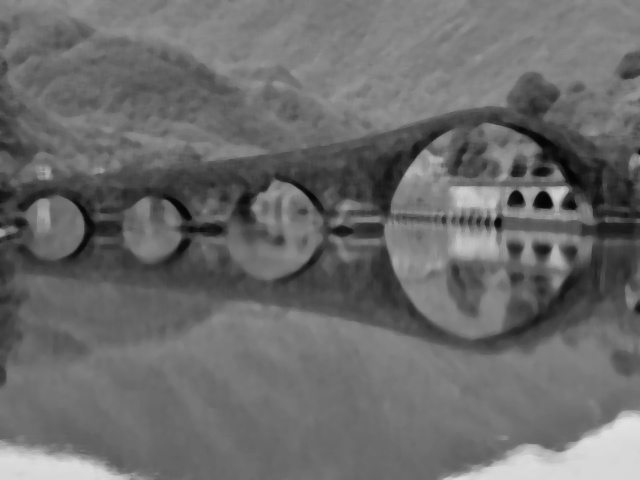
\epsfig{file=kepek/graymedian.jpg,scale=0.5}
\caption{Szürkére átalakított kép medián szűrővel} 
\label{fig:cartoon3}
\end{figure}

\newpage

\SubSection{Adaptív küszöbölés az élek kiemelésére}

Az adaptív küszöbérték általában szürkeárnyalatos vagy színes képet kap bemenetként, és a legegyszerűbb megvalósításban bináris képet eredményez. A kép minden egyes képpontjára egy küszöbértéket kell kiszámítani. Ez a küszöbérték lehet például egy kernelen belüli intenzitások átlaga, vagy egy, a hisztogram alapján becsült érték. Amennyiben a képpontérték a küszöbérték alatt van, akkor a háttérértékre van állítva, ellenkező esetben az előtérbe kerül.

\begin{figure}[h!]
\centering
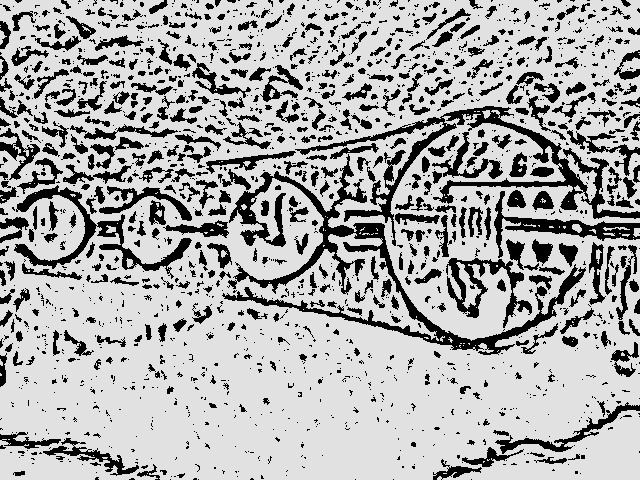
\epsfig{file=kepek/threshold.jpg,scale=0.5}
\caption{Az adaptív küszöbölés eredménye} 
\label{fig:cartoon4}
\end{figure}

\SubSection{A szűrőkkel és a küszöböléssel előállított képek egyesítése}

Az adaptív küszöböléssel elkészült maszkot át kell konvertálni színes képpé, hogy egyesíteni tudjuk az "elmosott" képpel amit az első két lépésben hoztunk létre. Ennek az elvégzését követően \aref{fig:cartoon5}. ábrán látható eredményt kaptuk.

\begin{figure}[h!]
\centering
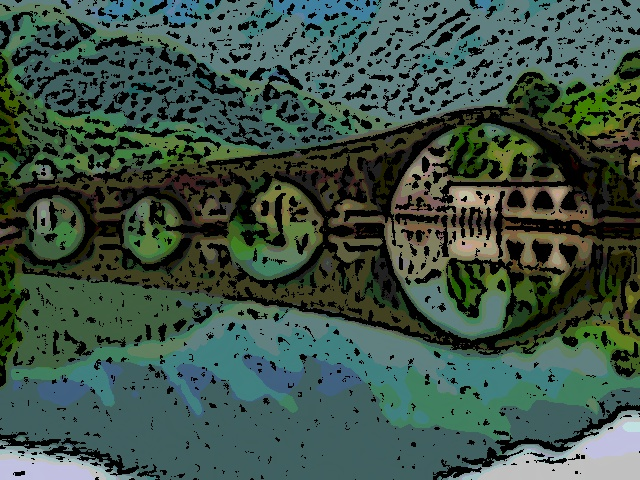
\epsfig{file=kepek/Cartoon_filter.jpg,scale=0.65}
\caption{Cartoon-style szűrő } 
\label{fig:cartoon5}
\end{figure}

% TODO: Esetleg pontszerű zajok eltávolítási módjáról lehet még néhány dolog a binarizált kép esetében.

\Section{Pencil sketch filter}

% https://github.com/MasteringOpenCV/code/blob/master/Chapter1_AndroidCartoonifier/Cartoonifier_Desktop/cartoon.cpp

Megpróbáltam egy olyan algoritmust létrehozni, ami egy ceruza rajzot imitál. A szakirodalomban találunk hasonló szűrési eljárásokat, mivel egy gyakran előforduló hatásról van szó \cite{beyeler2}.

A feldolgozáshoz szűrkeárnyalatosra konvertáltam a képet, medián szűrőt, Gauss szűrőt és egyéb képfeldolgozási műveleteket használtam, valamint egy "vásznat" is ráraktam, hogy még jobban olyan érzete legyen a képnek mint ha rajzolták volna (\ref{fig:pencil1}. ábra).

\begin{figure}[h!]
\centering
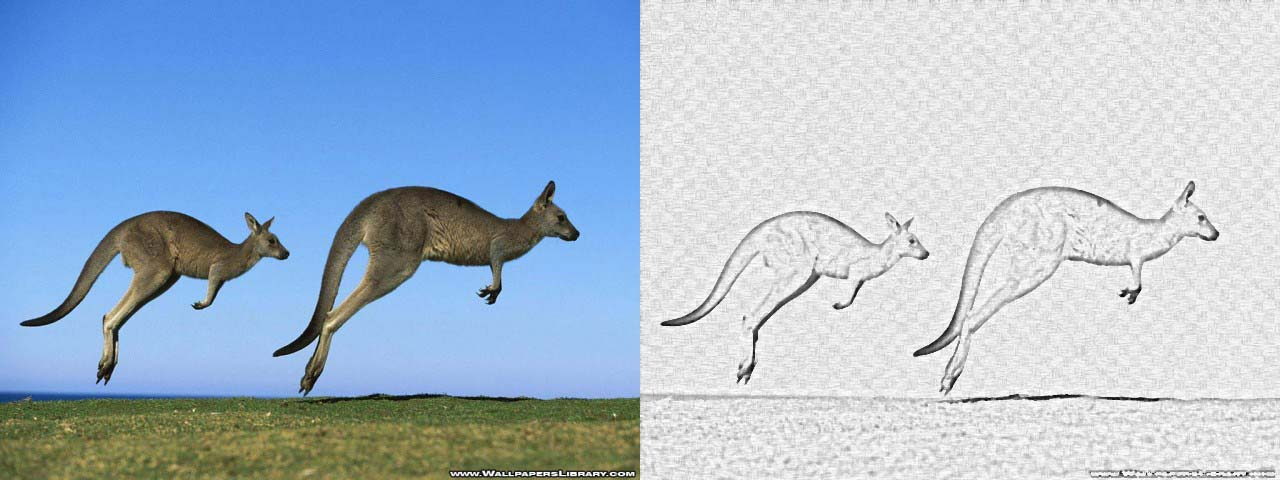
\epsfig{file=kepek/2_pencil_sketch_filter.jpg,width=15cm, height=5.625cm}
\caption{Bal oldalon az eredeti kép látható, jobb oldalon a filterrel ellátott kép $\quad$ (forrás: \textit{https://amazing.zone/kangaroos/they-only-can-go-forward})} 
\label{fig:pencil1}
\end{figure}

\newpage

\SubSection{Medián szűrő}

A kép szűrkeárnyalatos konvertálása után, végrehajtottam egy medián szűrést a kisebb, pont szerű zajok eltávolítása céljából (\ref{fig:pencil2}. ábra). A kernel méretétől függően már ez ad egy enyhe elmosást is a képhez, amely a végeredmény szempontjából előnyös.

\begin{figure}[h!]
\centering
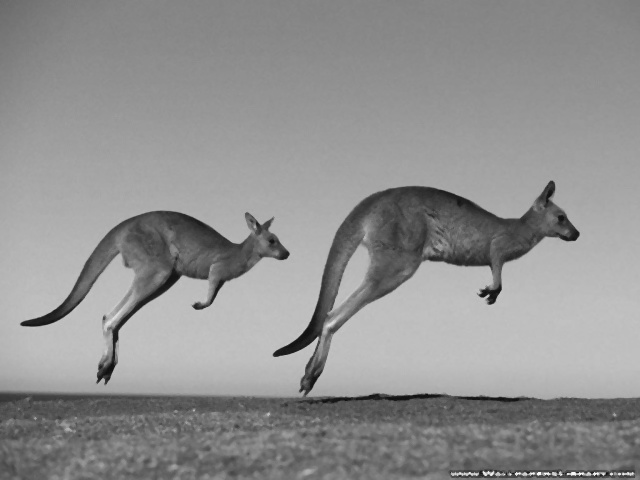
\epsfig{file=kepek/mediangray.jpg,scale=0.50}
\caption{Szürkére átalakított kép medián szűrővel} 
\label{fig:pencil2}
\end{figure}

\SubSection{Gauss szűrő}

Ezt a simítási teknikát, a képzaj  és a részletesség csökkentése érdekében használtam. Olyan sima elmosódást eredményez a képen, mint ha az nem lenne fókuszban (\ref{fig:pencil3}. ábra). A medián szűrőhöz képest lényeges különbség, hogy ezzel új árnyalatok is megjelennek a képen, a kontraszt összességében csökken.

\begin{figure}[h!]
\centering
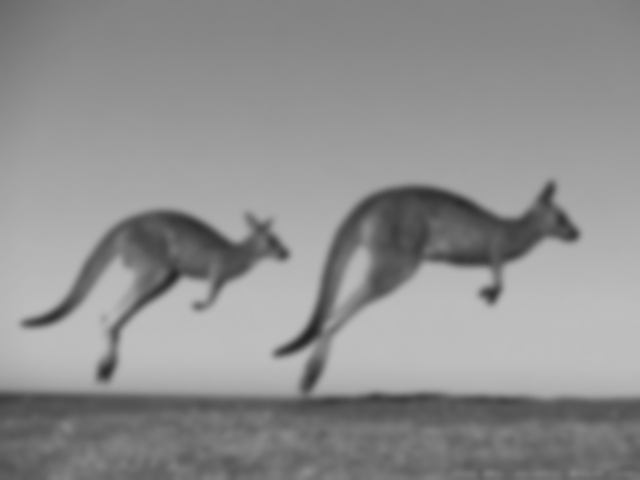
\epsfig{file=kepek/gauss.jpg,scale=0.5}
\caption{Gauss szűrő használata } 
\label{fig:pencil3}
\end{figure}

\SubSection{Az előző két lépés elosztása}

% TODO: Az osztást itt részletezni kicsit!

Az előző két szűrőt elosztottam egymással, így már tényleg majdnem olyan képet kaptam ami már ceruza rajz szerű. Úgy gondoltam még azért ráfér némi javítás, így még további műveleteket hajtottam végre rajta.

\begin{figure}[h!] 
\centering
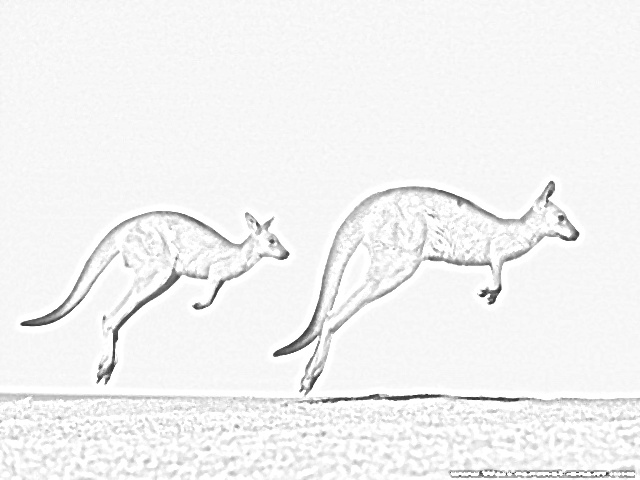
\epsfig{file=kepek/blend.jpg,scale=0.5}
\caption{Medián szűrés és a Gauss szűrés hányadosa } 
\label{fig: pencil4}
\end{figure}

\SubSection{Kontraszt széthúzása}

Azt figyeltem meg, hogy ha így hagyom a "Pencil sketch" szűrőt, akkor némely kép eléggé kontraszt szegény marad. Emiatt célszerűnek tünt belerakni egy kontraszt széthúzást, a szebb végeredmény érdekében. A széthúzás (vagy másnéven \textit{normalizáció}) egy egyszerű képjavító eljárás, amely megpróbálja javítani a kép kontrasztját azáltal, hogy "kiterjeszti" a benne lévő intenzitásértékek tartományát a kívánt értéktartományra. Ezt a műveletet követően a példaként szereplő képre \aref{fig:pencil5}. ábrán látható eredményt kaptam.

\begin{figure}[h!]
\centering
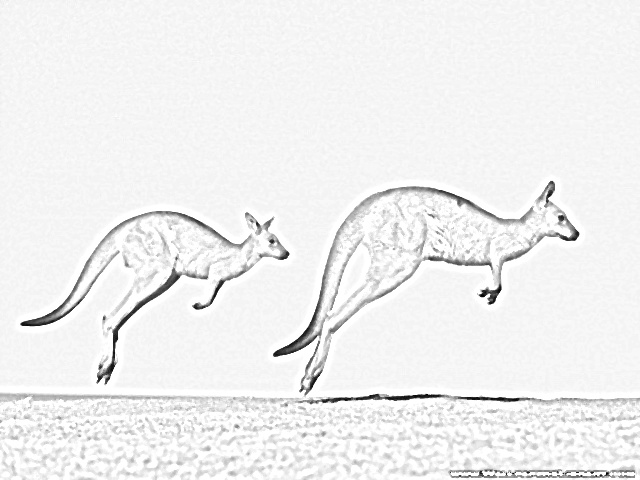
\epsfig{file=kepek/contraststrech.jpg,scale=0.5}
\caption{Kontraszt széthúzás} 
\label{fig:pencil5}
\end{figure}

\SubSection{Vászon hozzáadása}

A kontraszt széthúzása után, már egészen olyan hatása volt a képnek, mint ha egy ceruza rajz lenne. Ráraktam még egy "vászont" ami személyes véleményem szerint mégjobban segíti azt az érzetet hogy ez egy ceruzarajz. Először a vászonnak a színét át kellett konvertálnom színesből szűrkeárnyalatossá, hogy használható legyen a kontraszt széthúzott képhez (\ref{fig:pencil6}. ábra). Ezek után a vászont összeszoroztam az eddig eredményül kapott képpel, így jött létre a "Pencil sketch filter".

\begin{figure}[h!] 
\centering

\epsfig{file=kepek/canvasgray.jpg,scale=0.32}
\caption{Vászon színének konvertálása}
\label{fig:pencil6}
\end{figure}

\Aref{fig:pencil7}. ábrán láthatjuk a végeredményként kapott képet.

\begin{figure}[h!]
\centering
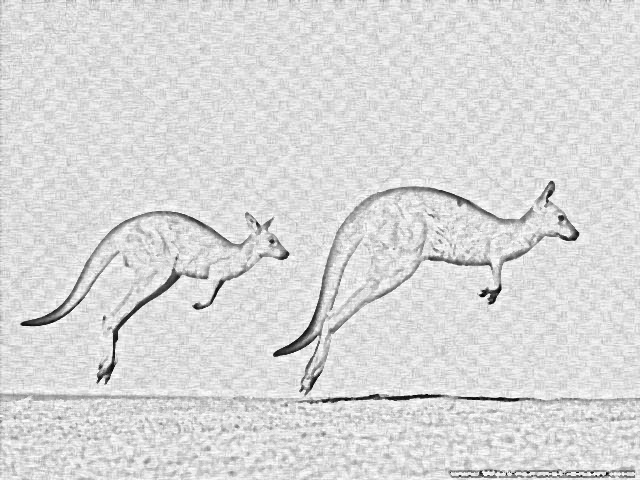
\epsfig{file=kepek/pencil_sketch.jpg, scale=0.4}
\caption{A \textit{Pencil sketch filter} eredménye} 
\label{fig:pencil7}
\end{figure}

\Section{Cartoon filter}

Megpróbáltam más technikával is létrehozni egy cartoon hatású képet, mivel a fellelhető irodalmakban is számos, különféle megoldást találni \cite{emami}.

Ahol medián szűrőt, Laplace éldetektálást valamit küszöbölést használtam (\ref{fig:2_cartoon1}. ábra).

\begin{figure}[h!]
\centering
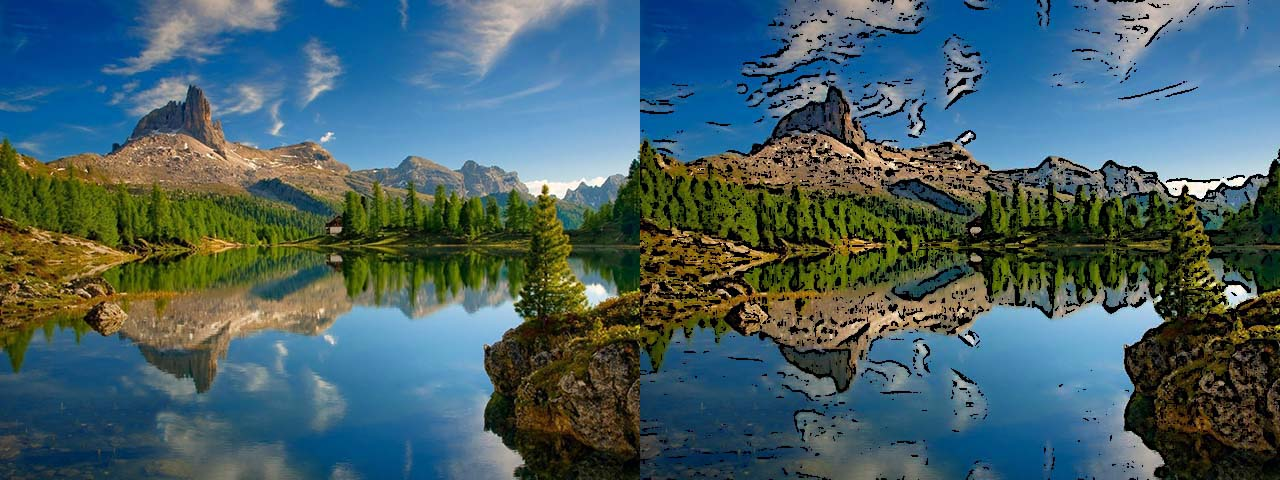
\epsfig{file=kepek/3_cartoon_filter2.jpg,width=15cm, height=5.625cm}
\caption{Bal oldalon az eredeti kép látható, jobb oldalon a filterrel ellátott kép $\quad$ (forrás: \textit{http://wallpaper-gallery.net/single/wallpaper-full-hd-nature/wallpaper-full-hd-nature-1.html})} 
\label{fig:2_cartoon1}
\end{figure}

\SubSection{Medián szűrő}

Mint az eddigi saját filtereknél, itt is előfeldolgozásként elvégeztem szürkeárnyalatossá konvertálást valamint egy medián szűrést (\ref{fig:2_cartoon2}. ábra).

\begin{figure}[h!]
\centering
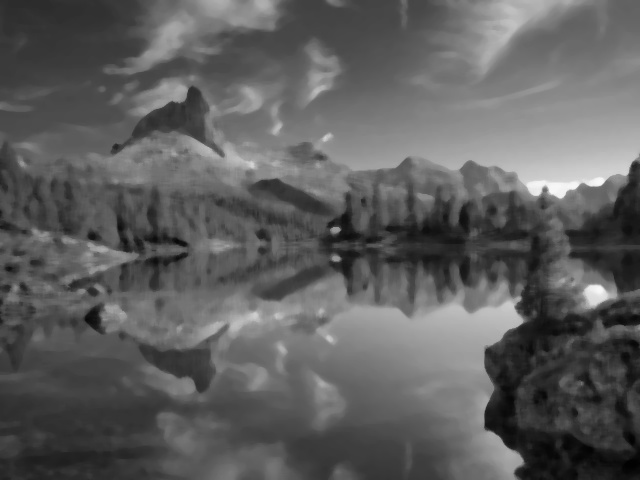
\epsfig{file=kepek/Cartoon1_gray.jpg,scale=0.45}
\caption{Szürkére átalakított kép medián szűrővel} 
\label{fig:2_cartoon2}
\end{figure}

\SubSection{Laplace éldetektálás}

Ennél a filternél a Laplace éldetektálást választottam. Ezzel olyan élmaszkot tudtam készíteni, amely kicsit hasonló a ceruza rajzhoz. Vékony kontúrként emeli ki a képben található éleket (\ref{fig:2_cartoon3}. ábra).

% Ez az éldetektálás gradiensekkel számol, ahol a gradiens nagy, ott a második derivált értéke 0.

\begin{figure}[h!]
\centering
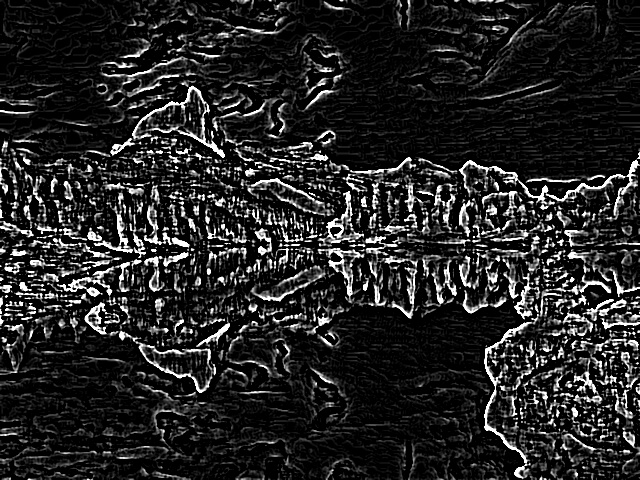
\epsfig{file=kepek/Cartoon1_laplacian.jpg,scale=0.45}
\caption{Laplace éldetektálás} 
\label{fig:2_cartoon3}
\end{figure}

\SubSection{Küszöbölés}

Az éldetektálás után, alkalmaztam egy küszöbölést amivel létrejött egy maszk, amit összeraktam az eredeti képpel (\ref{fig:2_cartoon4}. ábra).

\begin{figure}[h!]
\centering
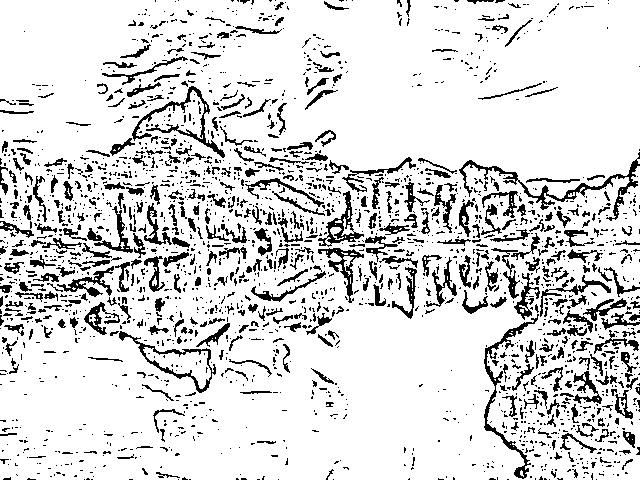
\epsfig{file=kepek/Cartoon1_thresh.jpg,scale=0.45}
\caption{Küszöbölés} 
\label{fig:2_cartoon4}
\end{figure}

Így készült el végeredményként a \textit{Cartoon filter}, melynek az eredménye \aref{fig:2_cartoon5}. ábrán látható.

\begin{figure}[h!]
\centering
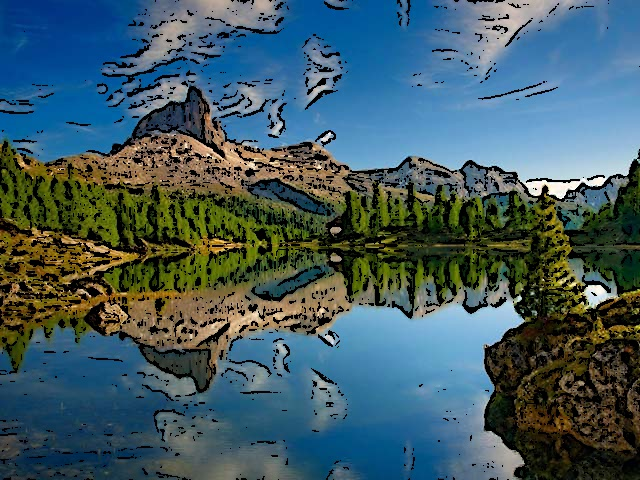
\epsfig{file=kepek/Cartoon1_filter1.jpg,scale=0.45}
\caption{Cartoon filter} 
\label{fig:2_cartoon5}
\end{figure}

\Section{Aquarelle-style filter}

Az utolsó saját szűrő amit készítettem az egy egyszerű vízfesték (\textit{aquarell}) hatású szűrő. Ez a szűrő teljesen más technikával készült mint az eddigiek. Nem használtam éldetektálást illetve küszöbölést sem. Az eredeti képpel dolgoztam végig, nem maszkoltam. A szűrés két lépésben megoldhatónak bizonyult. Elég egy átlagoló szűrés és egy mean shift szegmentálás egymást követően alkalmazni (\ref{fig:paint}. ábra).

\begin{figure}[h!]
\centering

\epsfig{file=kepek/4_paint_filter.jpg,width=15cm, height=5.625cm}
\caption{Aquarelle-style filter (forrás: \textit{https://marieclaire.hu/kultura/2015/11/24/nem-mindig-az-a-cel-hogy-a-nezo-jol-erezze-magat-interju-kokai-tundevel/})} 
\label{fig:paint}
\end{figure}

\SubSection{Átlagoló szűrő}

Átlagoló szűrővel elmostam az eredeti színes képet, hogy az apróbb zajokat kiszűrjem (\ref{fig:paint1}. ábra).

\begin{figure}[h!]
\centering

\epsfig{file=kepek/Paint_filter_blur.jpg,scale=0.48}
\caption{Átlagoló szűrő  } 
\label{fig:paint1}
\end{figure}

\SubSection{Mean shift szegmentálás}

Minden egyes adatpontnál a mean shift meghatároz egy ablakot, és kiszámítja az adatpont átlagát. Ezután az ablak közepét az átlag felé tolja, és megismétli az algoritmust, amíg konvergens. A mean shift egy nemparametrikus iteratív algoritmus vagy egy nemparametrikus sűrűségi gradiens becslés egy általánosított kernel megközelítés alkalmazásával (\ref{fig:paint2}. ábra).

\begin{figure}[h!]
\centering

\epsfig{file=kepek/Paint_filter.jpg,scale=0.6}
\caption{Aquarelle-style filter, mean shift szegmentálás  eredménye} 
\label{fig:paint2}
\end{figure}

% https://gist.github.com/dgym/5532135
% Ide kellene felsorolni majd a saját szűrők algoritmusait!

\end{comment}
% !TEX encoding = UTF-8 Unicode

\Chapter{SQL}
%\label{chap:implement}

\setlength{\parindent}{12.5mm}Alegtöbb adatbázis-kezelő rendszer az SQL szabványosított, vagy az alapján a saját rendszerhez finomhangolt nyelvet használja, így az oracle az Oracle SQL-t használja saját rendszerében. 


















\begin{comment}

\Section{OpenCV bemutatása}

Az OpenCV (Open Source Computer Vision Library) egy nyílt forráskódú számítógépes látás és gépi tanulási szoftverkönyvtár \cite{opencv}. Az OpenCV-t azért hozták létre, hogy közös infrastruktúrát biztosítson a számítógépes megjelenítési alkalmazások számára, és felgyorsítsa a gépi érzékelés használatát a kereskedelmi termékekben. BSD licenc alatt került kiadásra, ezért ingyenes mind tudományos, mind kereskedelmi célokra. C++, Python és Java interfészekkel rendelkezik, és támogatja a Windows, Linux, Mac OS, iOS és Android rendszereket. Az OpenCV-et a számítási hatékonyságra tervezték, és nagy hangsúlyt fektetett a valós idejű alkalmazásokra. Az optimalizált C/C++-ban írt, a könyvtár kihasználhatja a többmagos feldolgozást is. Az OpenCL használatával kihasználhatja az alapul szolgáló heterogén számítási platform hardveres gyorsítását.

A könyvtár több mint 2500 optimalizált algoritmussal rendelkezik, amely magába foglalja mind a klasszikus, mind a legmodernebb számítógépes látásmódot és a gépi tanulási algoritmusokat. Ezek az algoritmusok felismerhetik az arcokat, felismerhetik az objektumokat, osztályozhatják az emberi cselekvéseket a videókban, nyomon követhetik a mozgásokat, követhetik a mozgó objektumokat, eltávolíthatja a vörös szemeket a vakuval készített képekből, követheti a szemmozgásokat, felismerheti a tájat stb. 

% https://opencv.org

\Section{Beépített művészi jellegű OpenCV-s szűrők}

Az OpenCV könyvtár rendelkezik saját bepített, nem fotorealisztikus szűrőkkel, amelyeknél csak a bemeneti képet, valamint néhány paramétert kell megadnunk a függvénynek és ő elkészíti nekünk a filterezett képet. Négy ilyen beépített függvény található az OpenCV-ben, Edge Preserving filter, Detail Enhancing filter, Pencil sketch filter és a Stylization filter. Ezek C++ implementációját szeretném bemutatni.

\SubSection{Edge Preserving filter}

Az első ilyen szűrő az \textit{Edge Preversing filter}, ami az éleket megörzi de a hátteret elmossa (\ref{fig:edgePreservingFilter}. ábra). 
Ennek a paraméterezése az alábbi
\begin{cpp}
edgePreservingFilter(Mat src, Mat dst, int flags=1, 
                     float sigma_s=60, float sigma_r=0.4f);
\end{cpp}
szignatúrájú, ahol
\begin{itemize}
    \item \texttt{src}: a bemeneti kép, amit szeretnénk átalakítani,
    \item \texttt{dst}: a filterrel ellátot kép,
    \item \texttt{flags}: maga az élkiemelő filter melynek két paramétere lehet, \texttt{RECURS\_FILTER} (rekurív szűrő) aminek az értéke 1 vagy \texttt{NORMCONV\_FILTER} (normalizált konvolúció) aminek az értéke 2.  A futási sebességtől függ melyik paramétert alkalmazzuk, ha gyorsabb sebességet akarunk elérni akkor a rekurzív filtert érdemes használni, ha viszont nem számít a sebesség akkor a normalizált konvolúciót, mert az szebben kiemeli az éleket.
    \item \texttt{sigma\_s}: egy skálaérték 0 és 200 között (\textit{sigma spatial}), a simítás mértékét határozzuk meg vele,
    \item \texttt{sigma\_r}: egy skálaérték 0 és 1 között (\textit{sigma range}), azt szabályozza, hogy a szomszédságon belül a különböző színek milyen mértékben átlagolódjanak.
\end{itemize}

\begin{figure}[ht]
\centering
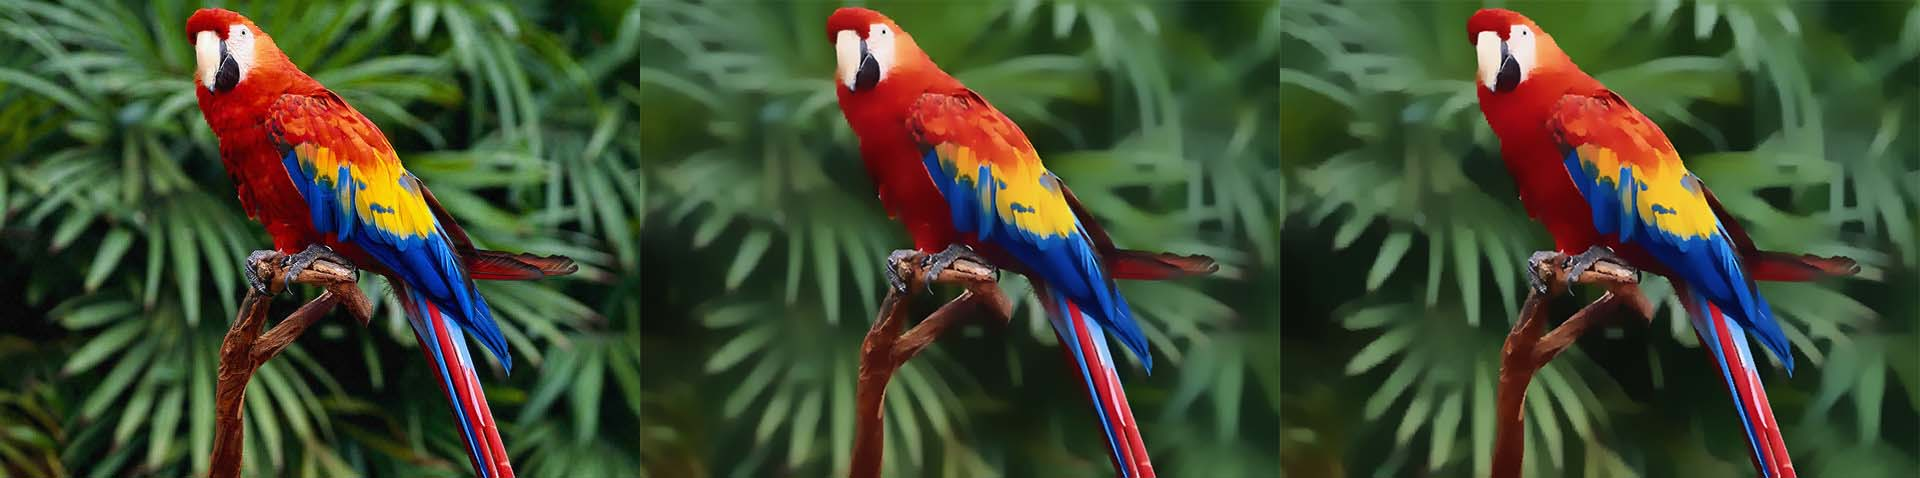
\epsfig{file=kepek/edgePreservingFilter.jpg,scale=0.45}
\caption{Eredeti kép, Rekurzív filter, Normalizált konvolúció $\hskip 4cm$ (forrás: \textit{https://sq.wikipedia.org/wiki/Papagalli})} 
\label{fig:edgePreservingFilter}
\end{figure}

\SubSection{Detail Enhancing filter}

A második ilyen szűrő a \textit{Detail Enhancing filter}, ami a képet élesebbé teszi (\ref{fig:detailEnhance}. ábra).
\begin{cpp}
detailEnhance(Mat src, Mat dst, float sigma_s=10, float sigma_r=0.15f);
\end{cpp}
A paraméterek megegyeznek az Edge Preserving filter paramétereivel. 

\begin{figure}[ht]
\centering
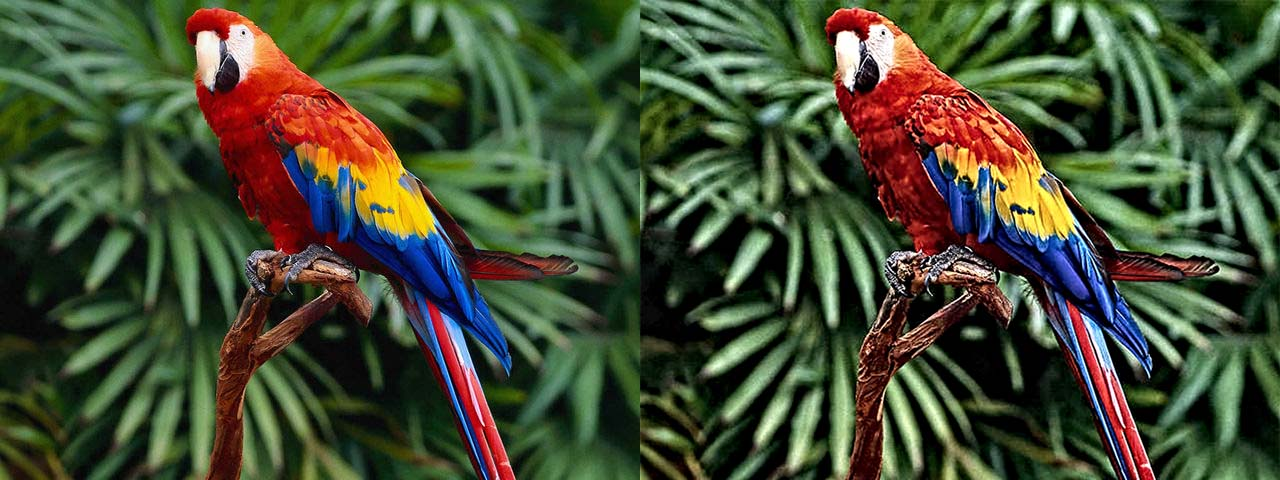
\epsfig{file=kepek/detailEnhance.jpg,scale=0.65}
\caption{Eredeti kép, Detail Enhancing filter eredménye} 
\label{fig:detailEnhance}
\end{figure}

\SubSection{Pencil sketch filter}

Ez a szűrő ceruza rajzot eredményez. Két féle képet is visszaad: egy színes képet és egy szürkeárnyalatosat (\ref{fig:pencil_sketch_color_grey}. ábra).
\begin{cpp}
pencilSketch(Mat src, Mat dst_gray, Mat dst_color, float sigma_s=60, 
             float sigma_r=0.07f, float shade_factor=0.02f);
\end{cpp}
A paraméterek megegyeznek az Edge Preserving szűrőével, de bővül az alábbi paraméterrel:
\begin{itemize}
    \item \texttt{shade\_factor}: ami egy 0 és 0,1 közötti érték, a kimeneti képintenzitás skálázása. Minél magasabb az érték, annál fényesebb az eredmény.
\end{itemize}

\begin{figure}[ht]
\centering
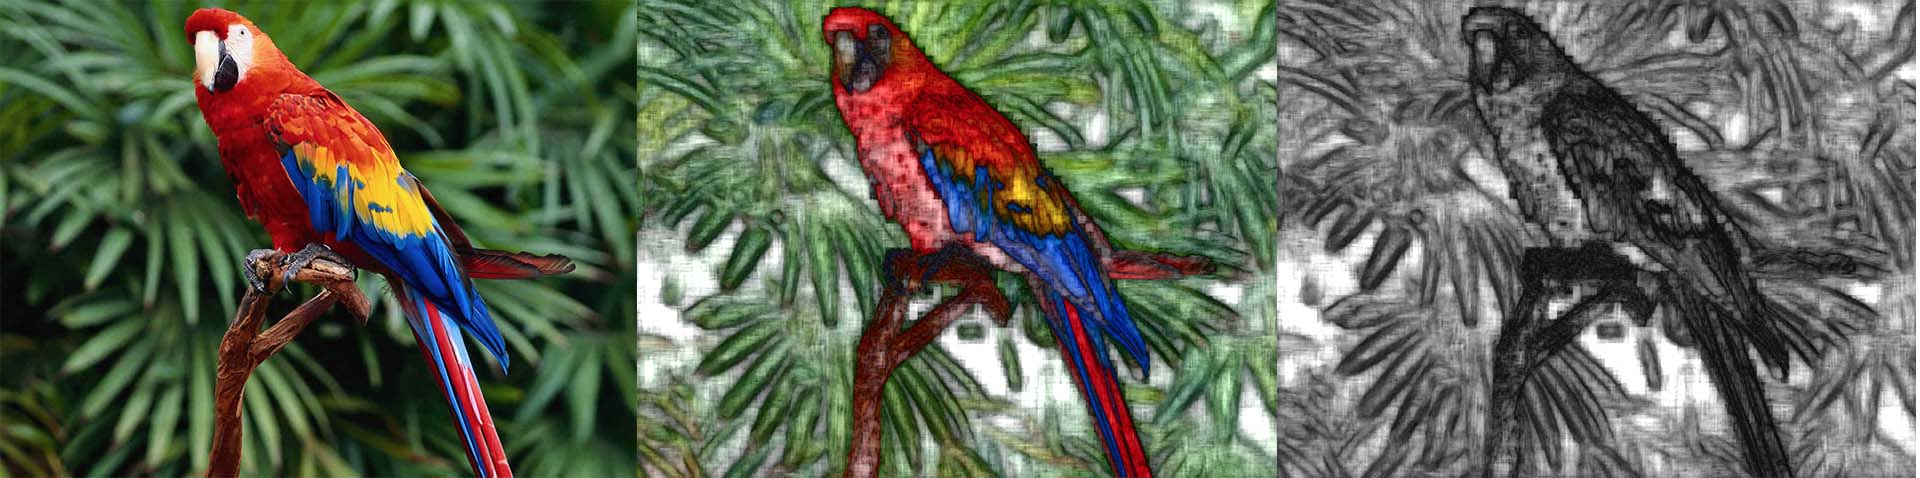
\epsfig{file=kepek/pencil_sketch_color_grey.jpg,scale=0.45}
\caption{Eredeti kép, Pencil sketch filter színes, Pencil sketch filter szűrkeárnyalatos} 
\label{fig:pencil_sketch_color_grey}
\end{figure}

\SubSection{Stylization filter}

A \textit{Stylization filter} olyan kimeneti képet eredményez, aminek olyan hatása van mint ha vízfestékkel készítették volna (\ref{fig:stylization}. ábra).
\begin{cpp}
stylization(Mat src, Mat dst, float sigma_s=60, float sigma_r=0.45f);
\end{cpp}
A paraméterek megegyeznek az Edge Preserving filter paramétereivel. 

\begin{figure}[ht]
\centering
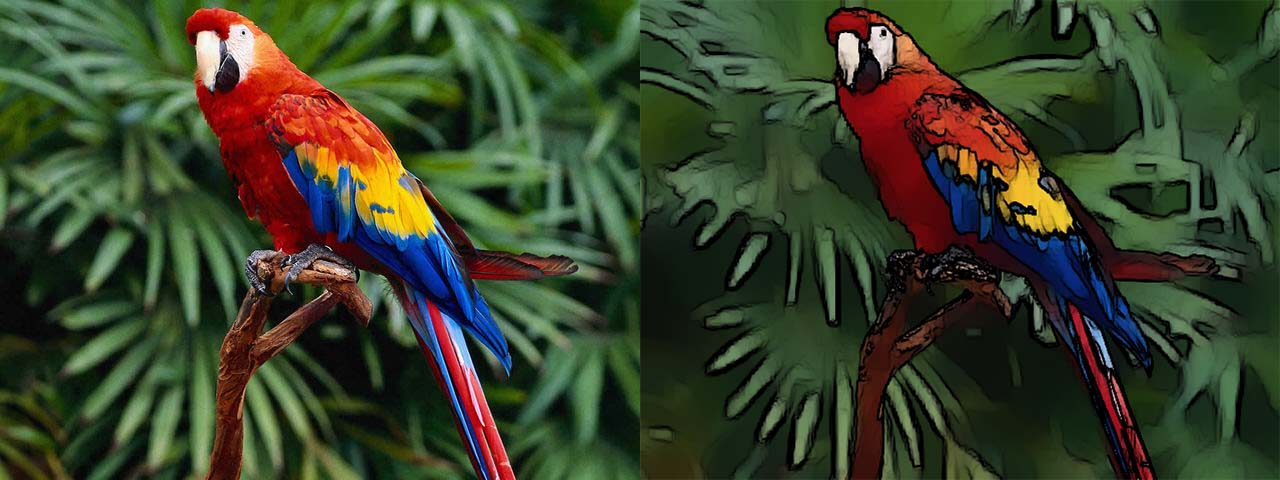
\epsfig{file=kepek/stylization.jpg,scale=0.65}
\caption{Eredeti kép, Stylization filter eredménye} 
\label{fig:stylization}
\end{figure}

%https://www.learnopencv.com/non-photorealistic-rendering-using-opencv-python-c/

\Section{Saját szűrők implementációja}

Ebben a fejezetben szeretném bemutatni a saját szűrőknek a C++ implementációját és a paramétereket amiket használtam hozzájuk. Ezeket itt már képekkel nem fogom illusztrálni, mert azok \aref{chap:filters}. fejezetben megtalálhatóak.

Elsőként bemutatnám a kép betöltésének implementációját, amit minden szűrőn használtam.
\begin{cpp}
Mat img = imread("image.jpg"); // bemeneti kep
Mat dst; // kimeneti kep
// Ha valami nem stimmel a kep betoltesnel
if (img.empty()) {
    cout << "Error loading the image" << endl;
    return -1;
}
\end{cpp} 
Az ablakok létrehozását a következőképpen oldottam meg:
\begin{cpp}
namedWindow("Original image", 1);
namedWindow("Image with filter", 1);
\end{cpp}
Ezután következik az a rész, amit a következő alfejezetekben fogok részletezni, hogy tulajdonképpen milyen lépésekből épül fel a filter. Ezek után a kép megjelenítése:
\begin{cpp}
imshow("Original imagel", img);
imshow("Image with filter", dst);
\end{cpp} 
\newpage
\noindent Végezetül a \texttt{waitKey} funkció következik, amely a megadott milliszekundumban megjeleníti a képet. Mivel itt nem mozgó képről beszélünk, így az értéke 0.
\begin{cpp}
waitKey(0);
\end{cpp}

\SubSection{Cartoon-style filter}

Ennek megvalósításához először a Gauss piramisban lefelé lépünk kettőt.
\begin{cpp}
for (int i = 0; i < 2; i++) {
    pyrDown(img, img);
}
\end{cpp}
A \texttt{pyrDown} függvény paraméterei:
\begin{itemize}
    \item \texttt{img}: a bemeneti színes kép,
    \item \texttt{img}: a kimeneti kicsinyített színes kép.
\end{itemize}
Egymás után hétszer hajtjuk végre a kétoldalú szűrőt az alábbi kód segítségével.
\begin{cpp}
Mat img_res;
int d = 9;
double sigmaColor = 9.0;
double sigmaSpace = 7.0;
for (int i = 0; i < 7; i++) {
    bilateralFilter(img, img_res, d, sigmaColor, sigmaSpace);
}
\end{cpp}
Ebben az
\begin{itemize}
    \item \texttt{img}: a bemeneti színes kép,
    \item \texttt{img\_res}: a kimeneti kép kétoldalú szűrővel,
    \item \texttt{d}: a szűrés során használt minden egyes pixel szomszédság átmérője. Ha nem pozitív, akkor kiszámítható a \texttt{sigmaSpace} értékéből,
    \item \texttt{sigmaColor}: szűri a szigmát a színtérben,
    \item \texttt{sigmaSpace}: szűri a szigmát a koordinátatérben.
\end{itemize}
Gauss piramisban felfelé lépünk kettőt, hogy visszanyerjük az eredeti kép méretet.
\begin{cpp}
for (int i = 0; i < 2; i++) {
    pyrUp(img_res, img_res);
}
\end{cpp}
amelynek a \texttt{pyrUp} függvényében az
\begin{itemize}
    \item \texttt{img\_res}: a bemeneti kép kétoldalú szűrővel,
    \item \texttt{img\_res}: a kimeneti nagyított színes kép.
\end{itemize}
Egy képet a
\begin{cpp}
cvtColor(img, srcGray, CV_BGR2GRAY);
\end{cpp}
utasítással konvertálhatunk szürkeárnyalatossá, amelyben
\begin{itemize}
    \item \texttt{img}: a bemeneti színes kép,
    \item \texttt{srcGray}: a kimeneti szürkeárnyalatos kép,
    \item \texttt{CV\_BGR2GRAY}: színes kép szürkeárnyalatosra alakítására használatos paraméter.
\end{itemize}
A következő lépésben a medián szűrőt implementáltam az
\begin{cpp}
int kernel_size = 7;
medianBlur(srcGray, median, kernel_size);
\end{cpp}
formában, ahol
\begin{itemize}
    \item \texttt{srcGray}: a bemeneti szürkeárnyalatos kép,
    \item \texttt{median}: a kimeneti medián szűrővel ellátott kép,
    \item \texttt{kernel\_size}: a kernel mérete, itt ebben az esetben egy $7 \times 7$-es mátrix. Ami már nem csak a zaj kiszűrését eredményezi, hanem már cartoon jellegűre mossa a képet.
\end{itemize}
Az adaptív küszöbölés implementációja az alábbi.
\begin{cpp}
Mat img_edge;
double maxValue = 225;
int blockSize = 9;
double C = 2; 
adaptiveThreshold(median,img_edge, maxValue, ADAPTIVE_THRESH_MEAN_C,
                  THRESH_BINARY, blockSize, C); 
\end{cpp}
amelyben
\begin{itemize}
    \item \texttt{median}: a bemeneti medián szűrővel ellátott kép,
    \item \texttt{img\_edge}: a kimeneti éldetektálás eredménye,
    \item \texttt{maxValue}: nem zérus érték hozzárendelve azokhoz a képpontokhoz, amelyekhez a feltétel teljesül.
    \item \texttt{ADAPTIVE\_THRESH\_MEAN\_C}: adaptiv küszöbölés algoritmus,
    \item \texttt{THRESH\_BINARY}: a küszöbérték típusának \texttt{THRESH\_BINARY} vagy \texttt{THRESH\_BINARY\_INV} értékűnek kell lennie,
    \item \texttt{blockSize}: a pixel szomszédságának mérete, amelyet a pixel küszöbértékének kiszámítására használnak,
    \item \texttt{C}: a konstanst az átlagból vagy a súlyozott átlagból kell levonni, normális esetben pozitív, de lehet nulla vagy negatív is.
\end{itemize}
A maszk színesre konvertálásához a
\begin{cpp}
cvtColor(img_edge, img_edge, CV_GRAY2RGB);
\end{cpp}
függvényt használhatjuk, ahol
\begin{itemize}
    \item \texttt{img\_edge}: a bemeneti szürkeárnyalatos kép,
    \item \texttt{img\_edge}: a kimeneti színes kép,
    \item \texttt{CV\_GRAY2RGB}: szürkeárnyalatos kép színesre alakítására használatos paraméter.
\end{itemize}
Az elmosott képet és a maszkot 
\begin{cpp}
Mat img_cartoon;
bitwise_and(img_res, img_edge, img_cartoon);
\end{cpp}
programsorokkal egyesíthetjük, ahol
\begin{itemize}
    \item \texttt{img\_res}: a bemeneti elmosott kép,
    \item \texttt{img\_edge}: a bemeneti élmaszk,
    \item \texttt{img\_cartoon}: kimeneti Cartoon-style filterezett kép.
\end{itemize}

\SubSection{Pencil sketch filter}

Első lépésként átkonvertáltam a képet színesről szűrkeárnyalatossá majd egy medián szűrést hajtottam végre. Ezt az előző szűrőnél már bemutattam így itt nem részletezném, annyiban változik a paraméterezése, hogy a kernel mérete itt egy $3 \times 3$-as mátrix.
A következő lépésben egy Gauss simítást implementáltam. 
\begin{cpp}
Mat gauss;
Size ksize = Size(21, 21);
double sigmaX = 0;
double sigmaY = 0;
GaussianBlur(median, gauss, ksize, sigmaX, sigmaY);
\end{cpp}
A \texttt{GaussianBlur} függvény paraméterezésében
\begin{itemize}
    \item \texttt{median}: a bemeneti medián szűrővel ellátott kép,
    \item \texttt{img\_blur}: a kimeneti Gauss szűrés eredménye,
    \item \texttt{ksize}: a kernel mérete, itt ebben az esetben egy $21 \times 21$-es mátrix,
    \item \texttt{sigmaX}: a Gauss kernel standard elterese $x$ iranyba,
    \item \texttt{sigmaY}: a Gauss kernel standard elterese $y$ iranyba.
\end{itemize}
A medián és Gauss szűrő elosztása egymással.
\begin{cpp}
Mat img_blend;
double scale_d = 245;
divide(median, gauss, img_blend, scale_d);   
\end{cpp}
A \texttt{divide} függvényben
\begin{itemize}
    \item \texttt{median}: a bemeneti medián szűrővel ellátott kép,
    \item \texttt{img\_blur}: a bemeneti Gauss szűrővel ellátott kép,
    \item \texttt{img\_blend}: a kimeneti kép a szűrők elosztásának eredménye,
    \item \texttt{scale\_d}: a skalár tényező.
\end{itemize}
Ezt követően kontraszt széthúzást alkalmaztam az alábbi kóddal.
\begin{cpp}
double alpha = 0;
double beta = 255;
normalize(img_blend, img_blend, alpha, beta, CV_MINMAX);
\end{cpp}
A \texttt{normalize} függvény paraméterei:
\begin{itemize}
    \item \texttt{img\_blend}: a két szűrő elosztásával kapott kép,
    \item \texttt{img\_blend}: a kimeneti kontraszt széthúzással kapott kép,
    \item \texttt{alpha}: normál érték a normálértékhez viszonyítva vagy az alsó tartomány határértéke esetén,
    \item \texttt{beta}: első tartományhatár a tartomány normalizálása esetén,
    \item \texttt{CV\_MINMAX}: választható maszk művelet.
\end{itemize}
A szürkeárnyalatos vászon összeszorzása a kontraszt széthúzott képpel való összeszorzása:
\begin{cpp}
double scale_m = 1.0 / 256;
multiply(img_blend, canvas, img_blend, scale_m);
\end{cpp}
ahol
\begin{itemize}
    \item \texttt{img\_blend}: a bemeneti kontraszt széthúzással ellátott kép,
    \item \texttt{canvas}: a bemenet vászon képe,
    \item \texttt{img\_blend}: a kimeneti összeszorzott kép,
    \item \texttt{scale\_m}: választható skálafaktor.
\end{itemize}

\SubSection{Cartoon filter}

Első lépésként itt mint az előző filtereknél, átkonvertáltam a képet színesről szűrkeárnyalatossá majd egy medián szűrést hajtottam végre, ahol a kernel mérete $7 \times 7$-es matrix.
Ezt egy Laplace éldetektálás követte.
\begin{cpp}
int kernel_size = 5;  
Laplacian(median, edges, CV_8U, kernel_size);
\end{cpp}
A \texttt{Laplacian} függvény paraméterei:
\begin{itemize}
    \item \texttt{median}: a bemeneti median szűrővel ellátott kép,
    \item \texttt{edges}: az élekdetektálás eredménye,
    \item \texttt{CV\_8U}: unsigned 8bit/pixel, azaz egy pixel $[0, 255]$ egész értékű tartományban lehet,
    \item \texttt{kernel\_size}: a kernel mérete, itt ebben az esetben egy $5 \times 5$-ös mátrix. Azt mutatja meg mekkora legyen a maszkon az él mérete.
\end{itemize}
Végezetül a küszöbölés következett.
\begin{cpp}
double thresh = 90;
double maxval = 255;
threshold(edges, mask, thresh, maxval, THRESH_BINARY_INV);
\end{cpp}
Ebben az
\begin{itemize}
    \item \texttt{edges}: a bemeneti kép az élekdetektálás eredménye,
    \item \texttt{mask}: a küszöbölés eredménye,
    \item \texttt{thresh}: küszöbérték,
    \item \texttt{maxval}: a \texttt{THRESH\_BINARY} és a \texttt{THRESH\_BINARY\_INV} küszöbérték típusokhoz használható maximális érték,
    \item \texttt{THRESH\_BINARY\_INV}:
$$
mask(x, y) =
\begin{cases}
0, & \mbox{ha } edge(x, y) > thresh, \\
maxval, & \mbox{különben}.
\end{cases}
$$
\end{itemize}

\SubSection{Aquarelle-stlye filter}

Ez a filter két egyszerű lépésből áll. Az első az egy átlagoló szűrő.
\begin{cpp}
Size ksize = Size(3, 3);
blur(img, avg, ksize);
\end{cpp}
amelyben
\begin{itemize}
    \item \texttt{img}: a bemeneti színes kép,
    \item \texttt{avg}: a kimeneti elmosott kép,
    \item \texttt{ksize}: a kernel mérete, itt ebben az esetben egy $3 \times 3$-as mátrix.
\end{itemize}
Mean shift szegmentáció.
\begin{cpp}
Mat img_shifted;
double sp = 15;
double sr = 50;
pyrMeanShiftFiltering(avg, img_shifted, sp, sr);
\end{cpp}
ahol
\begin{itemize}
    \item \texttt{avg}: a bemeneti átlagolással elmosott színes kép,
    \item \texttt{img\_shifted}: a kimeneti mean shift szegmentálással előállított kép,
    \item \texttt{sp}: a térbeli ablak sugara,
    \item \texttt{sr}: a színablak sugara.
\end{itemize}

\end{comment}
%% !TEX encoding = UTF-8 Unicode

\Chapter{Tesztek, eredmények bemutatása}
\label{chap:tests}

Azokat a szűrőket amelyeket \aref{chap:filters}. fejezetben tárgyaltam, nem csak képek átalakítására használtam, hanem videókon is teszteltem. Ebben a fejezetben szeretném leírni ezzel kapcsolatban a tapasztalataimat.  Fontosnak tartottam, hogy a vizsgálatok a futási időkre is kitérjenek, ezért a feldolgozási lépések számítási idejét külön-külön lemértem.

A tesztekhez használt számítógép konfigurációja a következő:
\begin{itemize}
\item MacBook Pro 2014 mid,
\item 2.6 GHz Intel Core i5 processzor,
\item 8GB RAM,
\item Intel Iris 1536 MB grafikus kártya,
\item macOS High Sierra operációs rendszer.
\end{itemize}

\Section{Szűrők tesztelése képeken}

Először képeken teszteltem az elkészített szűrőket. Az első tesztekben azt mutatom meg, hogy mennyi milliszekundum alatt készül el a kép és melyik művelet mennyi ideig tart, szintén milliszekundumban megadva.

A teszteknél a cél az, hogy megmutassa a korábban vizsgált szűrők számítási idejét. Ehhez az eddigi képek kerültek felhasználásra. A bemutatott példák számítási idejeit láthatjuk a következő szakaszokban.

\newpage

\SubSection{Cartoon-style filter}

A szűrő egyes lépéseinek időigényét \aref{fig:pie1}. ábrán láthatjuk. Az aktuális program esetében jól láthatóan időigényes művelet volt a kép betöltése, illetve a megjelenítéshez az ablak létrehozása.

A lényegi lépések közül a bilaterális szűr alkalmazása vette el a legtöbb időt, majd a szürkeárnyalatosra alakítás.

% Image loading time ms: 4.795\\
% Creating windows time in ms: 48.967\\
% Gaussian pyramid down in ms: 1.114\\
% Bilateral filter time in ms: 22.23\\
% Gaussian pyramid up time in ms: 1.387\\
% Convert rgb img to gray and median filter  time in ms: 8.844\\
% Adaptive threshold time in ms: 1.077\\
% Convert back to color, bit-AND time in ms: 2.813\\
% Write and show images time in ms: 21.723\\
% Image processing time in ms: 113.229\\\\

\begin{figure}[h!]
\centering
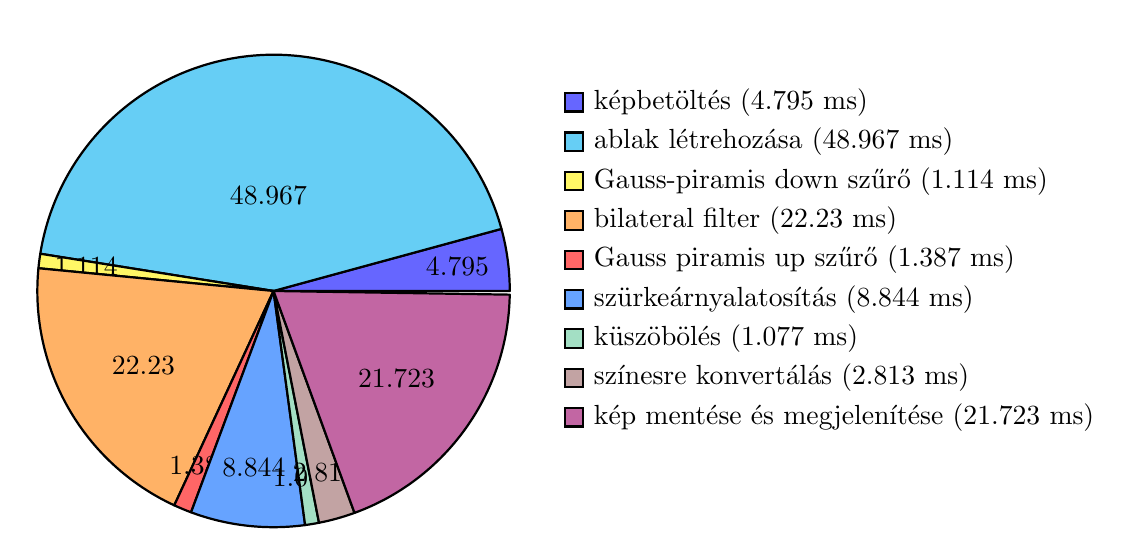
\begin{tikzpicture}
\pie[text=legend, sum=113.229]{
    4.795/képbetöltés (4.795 ms),
    48.967/ablak létrehozása (48.967 ms),
    1.114/Gauss-piramis down szűrő (1.114 ms),
    22.23/bilateral filter (22.23 ms),
    1.387/Gauss piramis up szűrő (1.387 ms),
    8.844/szürkeárnyalatosítás (8.844 ms),
    1.077/küszöbölés (1.077 ms),
    2.813/színesre konvertálás (2.813 ms),
    21.723/kép mentése és megjelenítése (21.723 ms)
}
\end{tikzpicture}
\caption{Cartoon style filter alkalmazásának időigénye (összesen 113.229 ms)}
\label{fig:pie1}
\end{figure}

\SubSection{Pencil sketch filter}

A szűrő szemléltetésére készített alkalmazás futásának jelentős idejét itt is a kép betöltése és az ablak megjelenítése tette ki (\ref{fig:pie2}. ábra). A következő nagyobb költségű művelet a Gauss szűrő alkalmazása volt.

% Image loading time in ms: 9.775\\
% Creating a window time in ms: 51.585\\
% Convert rgb iamge to gray and median filter time in ms: 1.495\\
% Gaussian filter time in ms: 9.691\\
% Gaussian filter and median filter divide time in ms: 0.476\\
% Contrast strech time in ms: 0.168\\
% Multiply the canvas and the smooth image time in ms: 2.793\\
% Write and show images time in ms: 17.503\\
% Image processing time in ms: 93.661

\begin{figure}[h!]
\centering
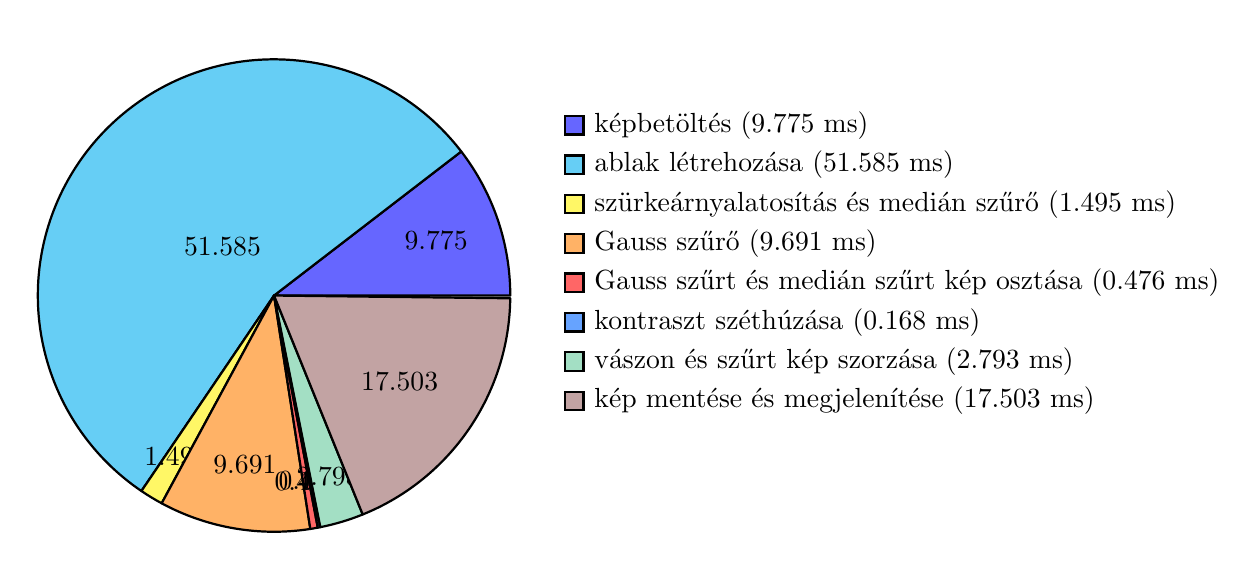
\begin{tikzpicture}
\pie[text=legend, sum=93.661]{
    9.775/képbetöltés (9.775 ms),
    51.585/ablak létrehozása (51.585 ms),
    1.495/szürkeárnyalatosítás és medián szűrő (1.495 ms),
    9.691/Gauss szűrő (9.691 ms),
    0.476/Gauss szűrt és medián szűrt kép osztása (0.476 ms),
    0.168/kontraszt széthúzása (0.168 ms),
    2.793/vászon és szűrt kép szorzása (2.793 ms),
    17.503/kép mentése és megjelenítése (17.503 ms)
}
\end{tikzpicture}
\caption{Pencil sketch filter alkalmazásának időigénye (összesen 93.661 ms)}
\label{fig:pie2}
\end{figure}

\SubSection{Cartoon filter}

A \textit{Cartoon filter} esetében láthatjuk, hogy a medián szűrés mennyire számításigényes művelet, mivel a kernelen belüli értékek rendezése szükséges hozzá (\ref{fig:pie3}. ábra). A Laplace élkiemelés, küszöbölés és a maszk alkalmazása is számítási időt tekintve lényegesen kisebb.

% Image loading time in ms: 4.959\\
% Create windows time in ms: 51.136\\
% Median filtering time in ms: 9.916\\
% Laplacian edge detectation time in ms: 0.961\\
% Thresholding time in ms: 0.467\\
% Copy mask to the image time in ms: 0.838\\
% Write and show images time in ms: 19.56\\
% Image processing time in ms: 88.059\\\\

\begin{figure}[h!]
\centering
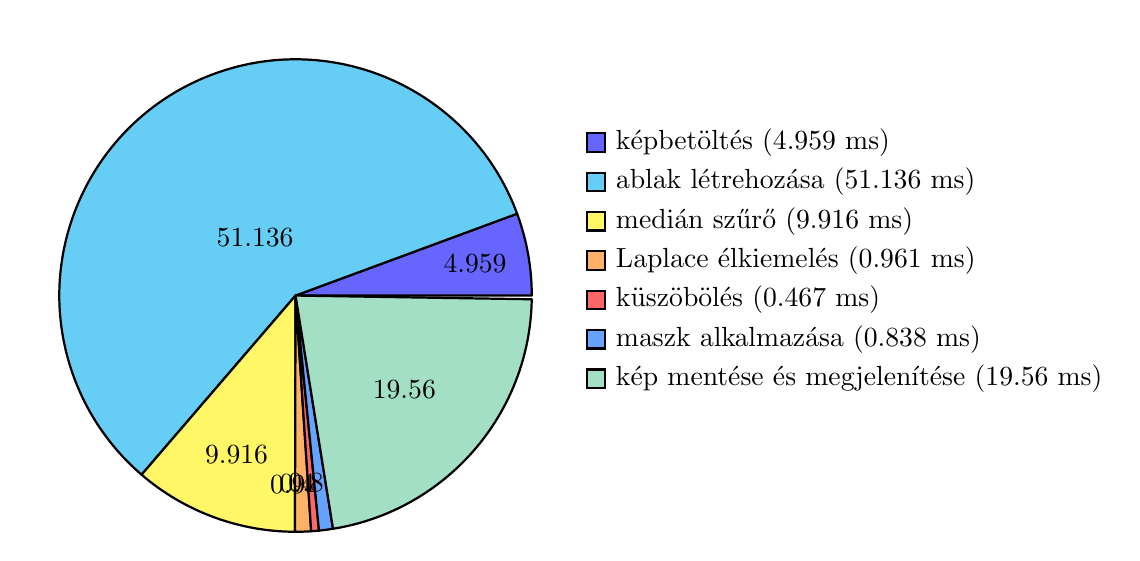
\begin{tikzpicture}
\pie[text=legend, sum=88.059]{
    4.959/képbetöltés (4.959 ms),
    51.136/ablak létrehozása (51.136 ms),
    9.916/medián szűrő (9.916 ms),
    0.961/Laplace élkiemelés (0.961 ms),
    0.467/küszöbölés (0.467 ms),
    0.838/maszk alkalmazása (0.838 ms),
    19.56/kép mentése és megjelenítése (19.56 ms)
}
\end{tikzpicture}
\caption{Cartoon filter alkalmazásának időigénye (összesen 88.059 ms)}
\label{fig:pie3}
\end{figure}

\SubSection{Aquarelle-style filter}

A vízfestékszerű hatáshoz használt \textit{mean shift} szegmentálás nagyon számításigényes művelet, ahogy az a feldolgozási lépések számítási idejéből látszik (\ref{fig:pie4}. ábra). Az előzőekhez képest ez a szűrő az, amelyik a legtöbb számítást vette igénybe.

% Image loading time in ms: 6.432\\
% Creating windows time in ms: 50.489\\
% Avarage blur time in ms: 1.26\\
% Mean shift segmentation time in ms: 483.213\\
% Write and show image time in ms: 13.407\\
% Image processing time in ms: 554.927

\begin{figure}[h!]
\centering
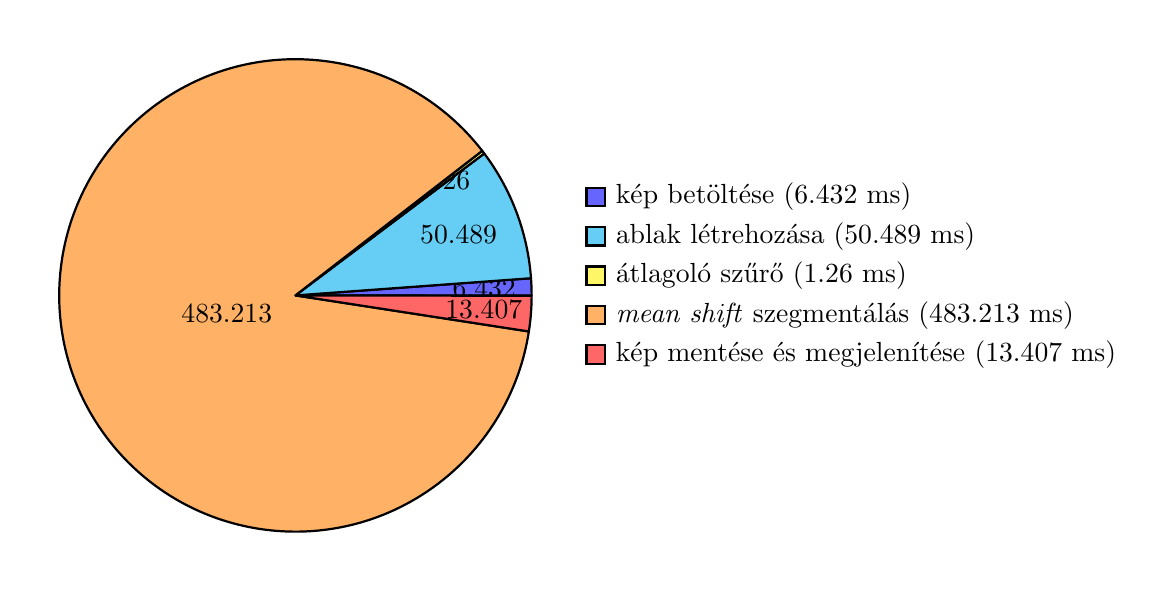
\begin{tikzpicture}
\pie[text=legend, sum=554.927]{
    6.432/kép betöltése (6.432 ms),
    50.489/ablak létrehozása (50.489 ms),
    1.26/átlagoló szűrő (1.26 ms),
    483.213/\textit{mean shift} szegmentálás (483.213 ms),
    13.407/kép mentése és megjelenítése (13.407 ms)
}
\end{tikzpicture}
\caption{Aquarelle-style filter alkalmazásának időigénye (összesen 554.927 ms)}
\label{fig:pie4}
\end{figure}

\Section{Szűrők tesztelése videókon és valós időben}

Ebben a részben, a videók valamint az élő kép feldolgozási idejét mérem képkocka per másodpercben, azaz fps-ben. Illetve az esetleges képi hibákról és azok kijavításási lehetőségeiről ejtek néhány szót.

\SubSection{Cartoon-style filter}

Ha futtatjuk az első filtert, látható, hogy a videó képe vibrál néhány pontban.

Ezeket ki lehet javítani, ha veszünk egy bizonyos kernel méretet és megvizsgáljuk, látjuk hogy a kernelen belül a színek túl nyomó többségben megegyeznek, viszont van néhány pont ami fekete, akkor a fekete pontokat átállítjuk olyan színüre, ami többségben van a kernelen belül. A videóknál, valamint a valós idejű feldolgozásnál mértem képkocka per másodpercet is. Látszik, hogy nem éri el a 24 fps-t sem a videó, sem a kamera képe ennél a szűrőnél. Azért 24 fps mivelt azt már az emberi szem folyamatosnak érzékeli, itt viszont kissé lassabb a kép. A méréseim alapján a videókon átlagosan 15-16 közötti képkocka szám van, a kamera képén 12-15.

\SubSection{Pencil sketch filter}

Számításaim alapján ez a szűrő volt az, ami már a videókon majdnem elérte a kellő fps számot, hogy folyamatos legyen. Itt videókon 20-21 között volt a képkocka szám, valós időben pedig 15-16. Itt nem volt annyira sok az egyes műveletek számítási ideje.

\SubSection{Cartoon filter}

Erről a szűrőről is elmondható ugyan az mint a Cartoon-style filterről, hogy a kép vibrál. Itt is alkalmazható lehetne az a megoldás, amit ott már leírtam. Itt a képkocka szám másodpercenként a videókban 17-18 között volt, valós időben 13-14 között.

\SubSection{Aquarelle-style filter}

Mint látható a képernyőnkön, ha futtatjuk a programot videóval vagy a saját kameránk képével eléggé "szaggat", vagyis a képkocka szám per másodperc, nagyon alacsony. Láthatjuk, hogy az előző képi tesztekben is ennek a szűrőnek volt a legnagobb feldolgozási ideje. A mean shift szegmentáció olyan mértékű számítás igényt jelent a programnak, hogy nem tudja teljesíteni a kívánt fps számot a számítógépem. Itt átlagosan a videón 3,2-3,5 közötti képkocka számot mértem, élő képen 2,5-2,8.

%FPS counter - https://ariandy1.wordpress.com/2013/02/19/calculating-fps-in-opencv-for-live-capture/
%4-6 oldal


%% !TEX encoding = UTF-8 Unicode

\Chapter{Összegzés}

A dolgozat a művészi szűrők témakörét mutatta be azok matematikai modelljén és néhány saját szűrő megvalósítás segítségével.

A dolgozat megírása előtt még nem foglalkoztam sem képfeldolgozással, sem azokkal az algoritmusokkal amelyeket itt említettem és használtam. Mindig is érdekelt, hogy ezek hogyan működnek. Az első pár hónapban komoly háttérkutatásokat végeztem, mind az algoritmusok és azok matematikai hátterével kapcsolatban.

Mint az előző fejezetekben olvasható, négy saját szűrőt raktam össze amelyek, rajzfilm, ceruzarajz-szerű, továbbá festmény jellegűek. Ezek mindegyikének bemutattam a matematikáját, valamint az implementációját. Néhányat ezek közül, leírások segítségével állítottam össze, de volt olyan amelyek teljesen saját ötlet alapján készült. A filterek algoritmusainak matematikai háttere az előző háttérkutatás után már nem volt ismeretlen, így már csak egy eszköz kellett, amivel meg is lehetett valósítani ezeket. 

Korábban nem használtam az OpenCV könyvtárat. A C++ programozási nyelv használata tünt a legcélszerűbbnek. (Eleinte C-ben kezdtem a kódok írását, de több olyan algoritmus implementációja hiányzik az OpenCV könyvtárból ami C++-ban viszont megtalálható. Ezen algoritmusokat viszont fontosak voltak a saját készítésű filterekhez.) Az algoritmusok a könyvtárban könnyedén használhatók, mint ahogy a \aref{chap:implement}. fejezetben részletezem. Egyszerűen megadjuk a kívánt paramétereket és már is elértük a kívánt műveletet.

Tesztekkel meg sikerült vizsgálni, hogy a szűrők használata során az egyes lépések számítási ideje milyen. Ezáltal jól láthatóvá váltak a képfeldolgozás szempontjából költségesebb műveletek. A videókon, továbbá a valós időben való képfeldolgozás a saját készítésű szűrők esetén néhány helyen még további kutatást és fejlesztést igényelne. A videók képe vibrál, ahogy \aref{chap:tests}. fejezetben is említettem, de akár látható is a dolgozathoz csatolt CD-mellékleten, ha futtatjuk ezen alkalmazásokat. Ezen hibák javítására szerepelnek javaslatok a dolgozatban, viszont javításukhoz egy külön, teljes körű, célzottan erre a problémakörre koncentráló kutatásra lenne szükség.

\newpage

\section*{Summary}

This work presents the topic of artistic filters, their mathematical foundations, and some of my own filter implementations. 

This is my first time working with image processing algorithms. I was always interested in how they work. In the first couple of months, I did background research about algorithms and their mathematical background. I have shown the results of this research in Chapter 3. 

I have designed and implemented four filters for cartoon, pencil and painting-like filtering. These filters take both theoretical and practical aspects into consideration. I have used the available literature, but the filters are based on my original ideas. Background research was conducted, mathematical formulas were given, and appropriate software tools were found for the implementation. 

I have never used the OpenCV library before. The usage of the C++ programming language seems to be the proper solution. (Initially, I started to code in C, but some algorithms are implemented in C++, which were necessary for my filters.) The algorithms of the library are easy to use, as we can see in Chapter 5. I have provided the appropriate parameters and reached the desired operation. 

I have checked the calculation time of the filtering steps, revealing the time consuming filtering operations. Some aspects of the video and real-time image processing require further research and development. The vibrating noise in the videos (as mentioned in Chapter 6 and can be checked by running the software) should be also filtered. I have proposed some solutions for reducing this type of noise, but their detailed consideration is out of the scope of this work.


% !TEX encoding = UTF-8 Unicode

\begin{thebibliography}{x}
\addcontentsline{toc}{chapter}{\bibname}

\bibitem{itu_ict_fac_fig_2017}
International Telecommunication Union: \emph{ICT Facts and Figures 2017}. International Telecommunication Union, 2017.

\bibitem{nav_online_szla}
Nemzeti Adó- és Vámhivatal, \emph{Online Számla}, \texttt{https://onlineszamla.nav.gov.hu}, Internet, 2018.

\bibitem{statcounter_os_market_share}
StatCounter, \emph{Operating System Market Share Hungary: July 2017 - July 2018},  \texttt{http://gs.statcounter.com/os-market-share/all/hungary}, Internet, 2018.

\bibitem{ecma_334_c_sharp}
ECMA International: \emph{ECMA-334 C\# Language Specification, 5th Edition}, ECMA International, 2017.

\bibitem{iso_iec_c_sharp_2006}
International Organization for Standardization, \emph{ISO/IEC 23270:2006(E), Second Edition}, International Organization for Standardization, 2006.

\bibitem{iso_iec_dis_c_sharp_future}
International Organization for Standardization, \emph{ISO/IEC DIS 23270}, \texttt{https://www.iso.org/standard/75178.html}, Internet, 2018.

\bibitem{ecma_335_cli_dotnet}
ECMA International: \emph{Common Language Infrastructure (CLI), 6th Edition}, ECMA International, 2012.

\bibitem{iso_iec_cli_dotnet_2012}
International Organization for Standardization, \emph{ISO/IEC 23271:2012(E), Third Edition}, International Organization for Standardization, 2012.

\bibitem{kovacs_laszlo_adatbazisok}
Kovács László: \emph{Adatbázisok tervezésének és kezelésének módszertana}, ComputerBooks, Budapest, 2004.

\bibitem{iso_iec_sql}
International Organization for Standardization, \emph{ISO/IEC 9075:2016, Fifth Edition}, International Organization for Standardization, 2016.

\bibitem{whats_new_in_sql}
Modern SQL: \emph{What's New in SQL:2016}, \texttt{https://modern-sql.com/blog/2017-06/whats-new-in-sql-2016}, Internet, 2017.










\begin{comment}

%innentol a vecsie!
\bibitem{intellipaint}
Reese, L. Jack, and William A. Barrett. \emph{Image editing with intelligent paint}. Proceedings of Eurographics. Vol. 21. No. 3. 2002.

\bibitem{instagram}
Instagram, hivatalos weboldal, \texttt{https://www.instagram.com/}, Internet, 2018.

\bibitem{snapchat}
Snapchat, hivatalos weboldal, \texttt{https://www.snapchat.com/}, Internet, 2018.

\bibitem{messenger}
Facebook messenger, hivatalos weboldal, \texttt{https://www.messenger.com/features}, Internet, 2018.

\bibitem{prisma}
Prisma, hivatalos weboldal, \texttt{https://prisma-ai.com/}, Internet, 2018.

\bibitem{pixect}
Pixect, hivatalos weboldal, \texttt{https://www.pixect.com/}, Internet, 2018.

\bibitem{jetset}
Smilebit: \emph{Jet Set Radio}, SEGA, \texttt{http://www.sega.com/games/jet-set-radio}, Internet, 2003.

\bibitem{scannerdarkly}
The New York Times, \emph{'A Scanner Darkly': Keanu Reeves, Undercover and Flying High on a Paranoid Head Trip}, 2006. július 7.

\bibitem{porthu}
Port.hu, \emph{Kamera által homályosan}, \texttt{https://port.hu/adatlap/film/tv/kamera-altal-\\homalyosan-a-scanner-darkly/movie-82437}, Internet, 2006.

\bibitem{czap}
Czap László: Képfeldolgozás, egyetemi jegyzet, Miskolci Egyetem, \\ \texttt{http://mazsola.iit.uni-miskolc.hu/~czap/HEFOP/Kepfeld1010.pdf}, 2007.

\bibitem{kato}
Kató Zoltán: Digitális képfeldolgozás, egyetemi kurzus, Szegedi Tudományegyetem, \texttt{http://www.inf.u-szeged.hu/~kato/teaching/DigitalisKepfeldolgozasTG}, 2014.

\bibitem{bilateral}
Paris, Sylvain, et al. \emph{A gentle introduction to bilateral filtering and its applications}. ACM SIGGRAPH 2007 courses. ACM, 2007.

\bibitem{sobel}
Utkarsh Sinha: \emph{The Sobel and Laplacian Edge Detectors}, \texttt{http://aishack.in/tutorials/sobel-laplacian-edge-detectors/}, 2010.

\bibitem{beyeler} Michael Beyeler: \emph{How to create a cool cartoon effect with OpenCV and Python}, \texttt{http://www.askaswiss.com/2016/01/} \texttt{how-to-create-cartoon-effect-opencv-python.html}, 2016. január 5.

\bibitem{beyeler2} Michael Beyeler: \emph{How to create a beautiful pencil sketch effect with OpenCV and Python}, \texttt{http://www.askaswiss.com/2016/01/} \texttt{how-to-create-pencil-sketch-opencv-python.html}, 2016. január 13.

\bibitem{emami} Shervin Emami: \emph{Mastering OpenCV with Practical Computer Vision Projects}, Packt Publishing, 2012.

\bibitem{opencv}
Bradski, Gary, and Adrian Kaehler. Learning OpenCV: \emph{Computer vision with the OpenCV library}. O'Reilly Media, Inc., 2008.

% TODO: Artistic filter-es könyv.

\end{comment}

\end{thebibliography}

% !TEX encoding = UTF-8 Unicode
\newpage
\section*{CD-melléklet tartalma}

A dolgozat PDF változatát a \texttt{dolgozat.pdf} fájlban találjuk.

A dolgozat \LaTeX\ segítségével készült. A forrásfájlok a \texttt{dolgozat} jegyzékben találhatók.

A dolgozathoz 4 művészi szűrő került implementálásra. Ezek a \texttt{filters} jegyzék alábbi aljegyzékeiben kaptak helyet.
\begin{itemize}
\item \texttt{cartoon-style}
\item \texttt{pencil-sketch}
\item \texttt{cartoon}
\item \texttt{aquarelle}
\end{itemize}

A példákban szereplő minták a forrásfájlok mellett találhatók. A program lefordítása után az közvetlenül kipróbálható.


\end{document}
